% Documents setup
\documentclass[11pt]{book}

% fix for pandoc 1.14
\providecommand{\tightlist}{%
  \setlength{\itemsep}{0pt}\setlength{\parskip}{0pt}}

\usepackage{tabu} % https://tex.stackexchange.com/questions/50332/vertical-spacing-of-a-table-cell

% Location of the csas-style repository: adjust path as needed
\newcommand{\locRepo}{csas-style}

% Use the style file in the csas-style repository (res-doc.sty)
\usepackage{\locRepo/res-doc}

% header-includes from R markdown entry
\setcounter{section}{1}

% Headers and footers
\lhead{Draft working paper --- Do not cite or circulate}
% \lhead{}
\rhead{}
% \rfoot{DRAFT - DO NOT CITE}

%%%% Commands for title page etc %%%%%

% Publication year
\newcommand{\rdYear}{2020}

% Publication month
\newcommand{\rdMonth}{}

% Report number
\newcommand{\rdNumber}{nnn}

% Region
\newcommand{\rdRegion}{Pacific Region}

% Title
\newcommand{\rdTitle}{Update to the assessment of Pacific Cod (\emph{Gadus macrocephalus}) for Hecate Strait and Queen Charlotte Sound (Area 5ABCD), and West Coast Vancouver Island (Area 3CD) in 2020}

% Author names separated by commas and ', and' for the last author in the format 'M.H. Grinnell' (use \textsuperscript{n} for addresses)
\newcommand{\rdAuth}{Robyn E. Forrest\textsuperscript{1}, Sean C. Anderson\textsuperscript{1}, Chris J. Grandin\textsuperscript{1}}

% Author names reversed separated by commas in the format 'Grinnell, M.H.'
\newcommand{\rdAuthRev}{Forrest, R.E., Anderson, S.C., and Grandin, C.J.}

% Author addresses (use \textsuperscript{n})
\newcommand{\rdAuthAddy}{\textsuperscript{1}Pacific Biological Station\\
Fisheries and Oceans Canada, 3190 Hammond Bay Road\\
Nanaimo, British Columbia, V9T 6N7, Canada\\}

\newcommand{\citationOtherLanguage}{}

% Name of file with abstract and resume (see \abstract and \frenchabstract for requirements)
\newcommand{\rdAbstract}{\abstract{The status of two stocks of Pacific Cod (\emph{Gadus macrocephalus}) in Hecate Strait/Queen Charlotte Sound (Area 5ABCD) and West Coast Vancouver Island (Area 3CD) was updated from the 2018 assessment, using Bayesian delay-difference models and data streams updated to 2019. The models were fit to fishery-independent indices of abundance and standardized commercial catch-per-unit-effort (CPUE) indices, updated from the 2018 stock assessment.}}

%%%% End of title page commands %%%%%

% \pdfcompresslevel=5 % faster PNGs

\setcounter{section}{0}

\bibliographystyle{csas-style/res-doc}

\usepackage{amsmath}
\usepackage{bm}

% commands and environments needed by pandoc snippets
% extracted from the output of `pandoc -s`
%% Make R markdown code chunks work
\usepackage{array}
\usepackage{amssymb,amsmath}
\usepackage{color}
\usepackage{fancyvrb}
\DefineShortVerb[commandchars=\\\{\}]{\|}
\DefineVerbatimEnvironment{Highlighting}{Verbatim}{commandchars=\\\{\}}
% Add ',fontsize=\small' for more characters per line
\newenvironment{Shaded}{}{}
\newcommand{\KeywordTok}[1]{\textcolor[rgb]{0.00,0.44,0.13}{\textbf{{#1}}}}
\newcommand{\DataTypeTok}[1]{\textcolor[rgb]{0.56,0.13,0.00}{{#1}}}
\newcommand{\DecValTok}[1]{\textcolor[rgb]{0.25,0.63,0.44}{{#1}}}
\newcommand{\BaseNTok}[1]{\textcolor[rgb]{0.25,0.63,0.44}{{#1}}}
\newcommand{\FloatTok}[1]{\textcolor[rgb]{0.25,0.63,0.44}{{#1}}}
\newcommand{\CharTok}[1]{\textcolor[rgb]{0.25,0.44,0.63}{{#1}}}
\newcommand{\StringTok}[1]{\textcolor[rgb]{0.25,0.44,0.63}{{#1}}}
\newcommand{\CommentTok}[1]{\textcolor[rgb]{0.38,0.63,0.69}{\textit{{#1}}}}
\newcommand{\OtherTok}[1]{\textcolor[rgb]{0.00,0.44,0.13}{{#1}}}
\newcommand{\AlertTok}[1]{\textcolor[rgb]{1.00,0.00,0.00}{\textbf{{#1}}}}
\newcommand{\FunctionTok}[1]{\textcolor[rgb]{0.02,0.16,0.49}{{#1}}}
\newcommand{\RegionMarkerTok}[1]{{#1}}
\newcommand{\ErrorTok}[1]{\textcolor[rgb]{1.00,0.00,0.00}{\textbf{{#1}}}}
\newcommand{\NormalTok}[1]{{#1}}
\newcommand{\OperatorTok}[1]{\textcolor[rgb]{0.00,0.44,0.13}{\textbf{{#1}}}}
\newcommand{\BuiltInTok}[1]{\textcolor[rgb]{0.00,0.44,0.13}{\textbf{{#1}}}}
\newcommand{\ControlFlowTok}[1]{\textcolor[rgb]{0.00,0.44,0.13}{\textbf{{#1}}}}

%Defines cslreferences environment
%Required by pandoc 2.8
%Copied from https://github.com/rstudio/rmarkdown/issues/1649

\DeclareGraphicsExtensions{.png,.pdf}
\begin{document}

\frontmatter
\begin{verbatim}
#> create.rdata.file: RData file found in C:/GitHub/pacific-cod-2020/models/0_1a_5ABCD_BASE_2020
#> 
#> create.rdata.file: RData file found in C:/GitHub/pacific-cod-2020/models/1_1a_3CD_BASE_2020
#> 
#> create.rdata.file: RData file found in C:/GitHub/pacific-cod-2020/models/0_1a_5ABCD_BASE_2020
#> 
#> create.rdata.file: RData file found in C:/GitHub/pacific-cod-2020/models/0_2d_5ABCD_rsoleq_1_1
#> 
#> create.rdata.file: RData file found in C:/GitHub/pacific-cod-2020/models/0_2e_5ABCD_q_cv06
#> 
#> create.rdata.file: RData file found in C:/GitHub/pacific-cod-2020/models/0_3a_5ABCD_Mprior_mean04_sd01
#> 
#> create.rdata.file: RData file found in C:/GitHub/pacific-cod-2020/models/0_5a_5ABCD_kage_3
#> 
#> create.rdata.file: RData file found in C:/GitHub/pacific-cod-2020/models/0_6b_5ABCD_sig015
#> 
#> create.rdata.file: RData file found in C:/GitHub/pacific-cod-2020/models/0_7b_5ABCD_sigW_015
#> 
#> create.rdata.file: RData file found in C:/GitHub/pacific-cod-2020/models/1_1a_3CD_BASE_2020
#> 
#> create.rdata.file: RData file found in C:/GitHub/pacific-cod-2020/models/1_2d_3CD_q_1
#> 
#> create.rdata.file: RData file found in C:/GitHub/pacific-cod-2020/models/1_2e_3CD_q_cv06
#> 
#> create.rdata.file: RData file found in C:/GitHub/pacific-cod-2020/models/1_3a_3CD_Mprior_mean04_sd01
#> 
#> create.rdata.file: RData file found in C:/GitHub/pacific-cod-2020/models/1_5a_3CD_kage3
#> 
#> create.rdata.file: RData file found in C:/GitHub/pacific-cod-2020/models/1_6b_3CD_sig015
#> 
#> create.rdata.file: RData file found in C:/GitHub/pacific-cod-2020/models/1_7b_3CD_sigW015
\end{verbatim}
\clearpage

\hypertarget{introduction}{%
\section{Introduction}\label{introduction}}

The last Pacific Cod assessment was conducted in 2018 (DFO \protect\hyperlink{ref-dfo2019}{2019}; Forrest et al. \protect\hyperlink{ref-forrest2020}{2020}). Separarat assessments were provided for stocks in Area 3CD and Area 5ABCD (Figure~\ref{fig:fig-map}). The assessment models were delay-difference models, fit to survey indices, commercial catch-per-unit-effort (CPUE), commercial catch data and commercial annual mean weights. Survey indices were available to 2016 for Area 3CD and 2017 for Area 5ABCD. Both stocks were assessed to be in the Cautious Zone (DFO \protect\hyperlink{ref-dfo2009}{2009}).

Since the last advice (DFO \protect\hyperlink{ref-dfo2019}{2019}), there has been no further request for science advice. However, it has recently come to our attention that the 2018 survey index for Area 3CD was very low, approximately 25\% of the previous two observations (Figure~\ref{fig:fig-wcvi-index-3cd}). The commercial CPUE index has also decreased since 2016 (Figure~\ref{fig:cpue-int-test-plot}). Catches in 2018 and 2019 in Area 3CD were also very low (Table~\ref{tab:tab-catch-3cd}, Figure~\ref{fig:fig-catch-3cd}).

While we did not see a decrease in survey or CPUE indices for either Hecate Strait or Queen Charlotte Sound (Figure~\ref{fig:surv-canadian}), which cover the Area 5ABCD stock, we have taken the opportunity to update all the data streams for both Areas 3CD and 5ABCD and re-run the stock assessment to re-assess stock status.
\begin{figure}[htb]

{\centering \pdftooltip{\includegraphics[width=6in]{knitr-figs/fig-wcvi-index-3cd-1}}{Figure \ref{fig:fig-wcvi-index-3cd}} 

}

\caption{West Coast Vancouver Island Synoptic Survey estimates, centred by geometric mean}\label{fig:fig-wcvi-index-3cd}
\end{figure}
\clearpage

\hypertarget{summary}{%
\section{Summary}\label{summary}}

We re-ran both the stock assessment models with identical settings to those used in 2018 (Forrest et al. \protect\hyperlink{ref-forrest2020}{2020}). For each area, we ran the reference model plus the six sensitivity cases that were selected by the 2019 Regional Peer Review (RPR) committee for inclusion in the model-averaged results (DFO \protect\hyperlink{ref-dfo2019}{2019}).

\hypertarget{data}{%
\subsection{Data}\label{data}}

Data were extracted from DFO databases in the same way as described in Forrest et al. (\protect\hyperlink{ref-forrest2020}{2020}), with updates to 2019. The models were fit to:
\begin{enumerate}
\def\labelenumi{\arabic{enumi}.}
\item
  Commercial catch data (Tables~\ref{tab:tab-catch-5abcd} and~\ref{tab:tab-catch-3cd}, Figures~\ref{fig:fig-catch-5abcd} and~\ref{fig:fig-catch-3cd});
\item
  Survey indices of abundance Figure~\ref{fig:surv-canadian}), where the 3CD model was fit to the WCVI Synoptic Survey and the NMFS triennial survey (Figure~\ref{fig:tri-fig9}, Vancouver Canadian series);
\item
  Historical (1956-1995) and modern (1996+) commercial CPUE indices (Figure~\ref{fig:cpue-int-test-plot}); and
\item
  Mean weight of Pacific Cod in the commercial bottom trawl fishery (see Forrest et al. (\protect\hyperlink{ref-forrest2020}{2020}) for details).
\end{enumerate}
\hypertarget{model-scenarios}{%
\subsection{Model scenarios}\label{model-scenarios}}

For Area 5ABCD, the scenarios (Sc) included in the model-averaging set were:

• Sc 1a Reference model.

• Sc 2d Set the mean of the prior probability distribution for synoptic survey ln(q) = ln(1.0) (pro-rated by depth-stratum areas of Area 5AB and 5CD).

• Sc 2e Increase the standard deviation (SD) for synoptic survey ln(q) to 0.6.

• Sc 3a Set the parameters of the prior probability distribution for ln(M) to mean = ln(0.4), SD = 0.1.

• Sc 5a Set knife-edged age at recruitment = 3 years.

• Sc 6b Reduce the overall observation error term \(\sigma_O\) = 0.15.

• Sc 7b Reduce the SD in the likelihood for the fit to average annual mean weight \(\sigma_W\) = 0.15.

For Area 3CD, the scenarios (Sc) included in the model-averaging set were:

• Sc 1a Reference model.

• Sc 2d Set the mean of the prior probability distribution for synoptic survey ln(q) = ln(1.0).

• Sc 2e Increase the standard deviation (SD) for synoptic survey ln(q) to 0.6.

• Sc 3a Set the parameters of the prior probability distribution for ln(M) to mean = ln(0.4), SD = 0.1.

• Sc 5a Set knife-edged age at recruitment = 3 years.

• Sc 6b Reduce the overall observation term \(\sigma_O\) = 0.15.

• Sc 7b Reduce the SD in the likelihood for the fit to average annual mean weight \(\sigma_W\) = 0.15.

See Forrest et al. (\protect\hyperlink{ref-forrest2020}{2020}) and DFO (\protect\hyperlink{ref-dfo2019}{2019}) for further details.

\hypertarget{reference-points}{%
\subsection{Reference points}\label{reference-points}}

As in the 2018 assessment (DFO \protect\hyperlink{ref-dfo2019}{2019}), historical reference points were used to assess stock status, where
\begin{enumerate}
\def\labelenumi{\arabic{enumi}.}
\item
  \(USR\) (Upper Stock Reference) is the historical mean of the biomass estimates from 1956--2004.
\item
  \(LRP\) (Limit Reference Point) is the lowest estimated biomass agreed upon as an undesirable state to be avoided. For Area 5ABCD this is the estimated biomass in 2000. For Area 3CD it is the estimated biomass in 1986.
\item
  \(LRR\) (Limit Removal Rate) is the average fishing mortality rate from 1956--2004.
\end{enumerate}
\hypertarget{sec:summary-results}{%
\subsection{Main Results}\label{sec:summary-results}}

We begin with a summary set of results for Area 3CD, followed by summary results for Area 5CD. A more complete set of tables and figures is provided in Sections~\ref{sec:tables} and~\ref{sec:figures}. However, we do not discuss these in detail.

The joint posterior distribution for each model was numerically approximated using the Markov Chain Monte Carlo (MCMC) routines built into AD Model Builder (Metropolis-Hastings algorithm) (Fournier et al. \protect\hyperlink{ref-fournier2012}{2012}). Posterior samples were drawn every 1,000 iterations from a chain of length 2 million, resulting in 2,000 posterior samples (the first 1,000 samples were dropped to allow for sufficient burn-in).

\emph{TODO: we could possibly provide some summary info on the detailed figs and tables if this document is of interest}

\hypertarget{area-3cd}{%
\subsection{Area 3CD}\label{area-3cd}}
\begin{figure}[htb]

{\centering \pdftooltip{\includegraphics[width=6in]{knitr-figs/summary-fig-base-catch-fit-3cd-1}}{Figure \ref{fig:summary-fig-base-catch-fit-3cd}} 

}

\caption{MPD fit to the catch data for Area 3CD reference model.}\label{fig:summary-fig-base-catch-fit-3cd}
\end{figure}
\begin{figure}[htb]

{\centering \pdftooltip{\includegraphics[width=6in]{knitr-figs/summary-fig-base-index-fits-3cd-1}}{Figure \ref{fig:summary-fig-base-index-fits-3cd}} 

}

\caption{MPD fits to observed indices of abundance (points) for the Area 3CD reference model from: (a) the West Coast Vancouver Island Synoptic Survey, (b) the Commercial CPUE pre-1996, (c) the Commercial CPUE post-1995, and (d) the NMFS Triennial Survey (Canadian portion).}\label{fig:summary-fig-base-index-fits-3cd}
\end{figure}
\begin{figure}[htb]

{\centering \pdftooltip{\includegraphics[width=6in]{knitr-figs/summary-fig-base-mean-weight-3cd-1}}{Figure \ref{fig:summary-fig-base-mean-weight-3cd}} 

}

\caption{MPD fit to the mean weight data for Area 3CD reference model.}\label{fig:summary-fig-base-mean-weight-3cd}
\end{figure}
\begin{figure}[htb]

{\centering \pdftooltip{\includegraphics[width=6in]{knitr-figs/summary-fig-base-biomass-3cd-1}}{Figure \ref{fig:summary-fig-base-biomass-3cd}} 

}

\caption{Posterior estimated biomass for the Reference Model, Area 3CD. The green dashed line shows the median Upper Stock Reference (USR) which is the mean biomass estimate for the years 1956--2004. The red dashed line shows the median Limit Reference Point (LRP) which is the lowest estimated biomass agreed to be an undesirable state to avoid, in this case it is the biomass estimate for 1986.}\label{fig:summary-fig-base-biomass-3cd}
\end{figure}
\begin{figure}[htb]

{\centering \pdftooltip{\includegraphics[width=6in]{knitr-figs/summary-fig-model-average-biomass-comp-3cd-1}}{Figure \ref{fig:summary-fig-model-average-biomass-comp-3cd}} 

}

\caption{Posterior estimates of biomass for the model-averaged set for Area 3CD. The green dashed line shows the median Upper Stock Reference (USR) which is the mean biomass estimate for the years 1956--2004. The red dashed line shows the median Limit Reference Point (LRP) which is the lowest estimated biomass agreed to be an undesirable state to avoid, in this case it is the biomass estimate for 1986.}\label{fig:summary-fig-model-average-biomass-comp-3cd}
\end{figure}
\clearpage
\begin{figure}[htb]

{\centering \pdftooltip{\includegraphics[width=6in]{knitr-figs/summary-fig-model-average-biomass-3cd-1}}{Figure \ref{fig:summary-fig-model-average-biomass-3cd}} 

}

\caption{Combined posterior biomass for the model-averaged set for Area 3CD.  The green dashed line shows the median Upper Stock Reference (USR) which is the mean biomass estimate for the years 1956--2004. The red dashed line shows the median Limit Reference Point (LRP) which is the lowest estimated biomass agreed to be an undesirable state to avoid, in this case it is the biomass estimate for 1986.}\label{fig:summary-fig-model-average-biomass-3cd}
\end{figure}
\clearpage
\begin{figure}[htb]

{\centering \pdftooltip{\includegraphics[width=6in]{knitr-figs/summary-fig-model-average-biomass-3cd-proj-1}}{Figure \ref{fig:summary-fig-model-average-biomass-3cd-proj}} 

}

\caption{Combined posterior estimates of biomass for the model-averaged set for Area 3CD with projections (to the end of 2019).  The upper horizontal green dashed line shows the median Upper Stock Reference (USR) which is the mean biomass estimate for the years 1956--2004. The lower horizontal red dashed line shows the median Limit Reference Point (LRP) which is the lowest estimated biomass agreed to be an undesirable state to avoid, in this case it is the biomass estimate for 2000. The coloured regions to the right of the vertical line represent projections based on various TACs. The line represents the posterior median and the shaded region represents the 95\% credible interval.For clarity, years before 2010 are removed.}\label{fig:summary-fig-model-average-biomass-3cd-proj}
\end{figure}
\clearpage

\hypertarget{sec:tables}{%
\section{TABLES}\label{sec:tables}}
\begin{longtable}[]{@{}lrrrrr@{}}
\caption{\label{tab:tab-catch-5abcd}Reported catch (mt) of Pacific Cod in Area 5ABCD by Canada and the USA, 1953--2020. The reported discards for the period 1953--1995 are unrepresentative of true discarding because the estimates were taken from logbooks. Discard estimates since 1996 are based on at-sea observations and are considered to be more representative of true discarding.}\tabularnewline
\toprule
\textbf{Year} & \textbf{Canada landed} & \textbf{Canada released at sea} & \textbf{Canada total} & \textbf{USA} & \textbf{Total catch}\tabularnewline
\midrule
\endfirsthead
\toprule
\textbf{Year} & \textbf{Canada landed} & \textbf{Canada released at sea} & \textbf{Canada total} & \textbf{USA} & \textbf{Total catch}\tabularnewline
\midrule
\endhead
1953 & 329 & 0 & 329 & 0 & 329\tabularnewline
1954 & 937 & 0 & 937 & 0 & 937\tabularnewline
1955 & 607 & 0 & 607 & 224 & 831\tabularnewline
1956 & 1,666 & 0 & 1,666 & 2,063 & 3,729\tabularnewline
1957 & 3,199 & 0 & 3,199 & 2,677 & 5,876\tabularnewline
1958 & 3,275 & 0 & 3,275 & 3,549 & 6,824\tabularnewline
1959 & 2,478 & 0 & 2,478 & 1,974 & 4,452\tabularnewline
1960 & 2,029 & 0 & 2,029 & 951 & 2,980\tabularnewline
1961 & 1,529 & 0 & 1,529 & 251 & 1,780\tabularnewline
1962 & 2,138 & 0 & 2,138 & 310 & 2,448\tabularnewline
1963 & 2,478 & 0 & 2,478 & 883 & 3,361\tabularnewline
1964 & 6,568 & 0 & 6,568 & 1,009 & 7,577\tabularnewline
1965 & 9,291 & 0 & 9,291 & 1,562 & 10,853\tabularnewline
1966 & 9,409 & 0 & 9,409 & 1,362 & 10,771\tabularnewline
1967 & 6,034 & 0 & 6,034 & 1,025 & 7,059\tabularnewline
1968 & 4,325 & 0 & 4,325 & 606 & 4,931\tabularnewline
1969 & 2,817 & 0 & 2,817 & 405 & 3,222\tabularnewline
1970 & 1,267 & 0 & 1,267 & 198 & 1,465\tabularnewline
1971 & 1,542 & 0 & 1,542 & 698 & 2,240\tabularnewline
1972 & 3,642 & 0 & 3,642 & 1,667 & 5,309\tabularnewline
1973 & 4,258 & 0 & 4,258 & 1,426 & 5,684\tabularnewline
1974 & 6,005 & 0 & 6,005 & 1,539 & 7,544\tabularnewline
1975 & 6,739 & 0 & 6,739 & 1,139 & 7,878\tabularnewline
1976 & 5,796 & 0 & 5,796 & 635 & 6,431\tabularnewline
1977 & 4,369 & 0 & 4,369 & 408 & 4,777\tabularnewline
1978 & 4,078 & 0 & 4,078 & 159 & 4,237\tabularnewline
1979 & 7,462 & 0 & 7,462 & 62 & 7,524\tabularnewline
1980 & 5,487 & 0 & 5,487 & 10 & 5,497\tabularnewline
1981 & 3,462 & 0 & 3,462 & 0 & 3,462\tabularnewline
1982 & 3,089 & 0 & 3,089 & 0 & 3,089\tabularnewline
1983 & 2,478 & 0 & 2,478 & 0 & 2,478\tabularnewline
1984 & 2,113 & 0 & 2,113 & 0 & 2,113\tabularnewline
1985 & 1,338 & 0 & 1,338 & 0 & 1,338\tabularnewline
1986 & 4,019 & 0 & 4,019 & 0 & 4,019\tabularnewline
1987 & 12,711 & 0 & 12,711 & 0 & 12,711\tabularnewline
1988 & 8,020 & 0 & 8,020 & 0 & 8,020\tabularnewline
1989 & 4,214 & 0 & 4,214 & 0 & 4,214\tabularnewline
1990 & 4,242 & 0 & 4,242 & 0 & 4,242\tabularnewline
1991 & 9,892 & 0 & 9,892 & 0 & 9,892\tabularnewline
1992 & 7,087 & 0 & 7,087 & 0 & 7,087\tabularnewline
1993 & 4,869 & 0 & 4,869 & 0 & 4,869\tabularnewline
1994 & 1,757 & 0 & 1,757 & 0 & 1,757\tabularnewline
1995 & 1,293 & 1 & 1,294 & 0 & 1,294\tabularnewline
1996 & 1,270 & 92 & 1,362 & 0 & 1,362\tabularnewline
1997 & 1,261 & 105 & 1,366 & 0 & 1,366\tabularnewline
1998 & 982 & 59 & 1,041 & 0 & 1,041\tabularnewline
1999 & 692 & 53 & 746 & 0 & 746\tabularnewline
2000 & 553 & 28 & 581 & 0 & 581\tabularnewline
2001 & 296 & 38 & 334 & 0 & 334\tabularnewline
2002 & 382 & 104 & 487 & 0 & 487\tabularnewline
2003 & 660 & 147 & 807 & 0 & 807\tabularnewline
2004 & 833 & 130 & 963 & 0 & 963\tabularnewline
2005 & 1,004 & 83 & 1,087 & 0 & 1,087\tabularnewline
2006 & 872 & 32 & 904 & 0 & 904\tabularnewline
2007 & 370 & 15 & 385 & 0 & 385\tabularnewline
2008 & 309 & 7 & 316 & 0 & 316\tabularnewline
2009 & 669 & 40 & 709 & 0 & 709\tabularnewline
2010 & 1,452 & 49 & 1,501 & 0 & 1,501\tabularnewline
2011 & 1,233 & 7 & 1,240 & 0 & 1,240\tabularnewline
2012 & 871 & 12 & 883 & 0 & 883\tabularnewline
2013 & 829 & 22 & 851 & 0 & 851\tabularnewline
2014 & 904 & 18 & 922 & 0 & 922\tabularnewline
2015 & 924 & 18 & 943 & 0 & 943\tabularnewline
2016 & 529 & 5 & 534 & 0 & 534\tabularnewline
2017 & 346 & 4 & 350 & 0 & 350\tabularnewline
2018 & 254 & 5 & 259 & 0 & 259\tabularnewline
2019 & 450 & 4 & 454 & 0 & 454\tabularnewline
\bottomrule
\end{longtable}
\clearpage
\begin{longtable}[]{@{}lrrrrr@{}}
\caption{\label{tab:tab-catch-3cd}Reported catch (mt) of Pacific Cod in Area 3CD by Canada and the USA, 1953--2020. The reported discards for the period 1953--1995 are unrepresentative of true discarding because the estimates were taken from logbooks. Discard estimates since 1996 are based on at-sea observations and are considered to be more representative of true discarding.}\tabularnewline
\toprule
\textbf{Year} & \textbf{Canada landed} & \textbf{Canada released at sea} & \textbf{Canada total} & \textbf{USA} & \textbf{Total catch}\tabularnewline
\midrule
\endfirsthead
\toprule
\textbf{Year} & \textbf{Canada landed} & \textbf{Canada released at sea} & \textbf{Canada total} & \textbf{USA} & \textbf{Total catch}\tabularnewline
\midrule
\endhead
1953 & 64 & 0 & 64 & 0 & 64\tabularnewline
1954 & 1,055 & 0 & 1,055 & 0 & 1,055\tabularnewline
1955 & 650 & 0 & 650 & 0 & 650\tabularnewline
1956 & 715 & 0 & 715 & 770 & 1,485\tabularnewline
1957 & 1,117 & 0 & 1,117 & 558 & 1,675\tabularnewline
1958 & 526 & 0 & 526 & 271 & 797\tabularnewline
1959 & 416 & 0 & 416 & 510 & 926\tabularnewline
1960 & 240 & 0 & 240 & 376 & 616\tabularnewline
1961 & 284 & 0 & 284 & 232 & 516\tabularnewline
1962 & 428 & 0 & 428 & 402 & 830\tabularnewline
1963 & 838 & 0 & 838 & 345 & 1,183\tabularnewline
1964 & 1,107 & 0 & 1,107 & 907 & 2,014\tabularnewline
1965 & 1,608 & 0 & 1,608 & 1,088 & 2,696\tabularnewline
1966 & 2,095 & 0 & 2,095 & 1,145 & 3,240\tabularnewline
1967 & 1,202 & 0 & 1,202 & 623 & 1,825\tabularnewline
1968 & 726 & 0 & 726 & 351 & 1,077\tabularnewline
1969 & 796 & 0 & 796 & 147 & 943\tabularnewline
1970 & 1,150 & 0 & 1,150 & 454 & 1,604\tabularnewline
1971 & 3,585 & 0 & 3,585 & 1,319 & 4,904\tabularnewline
1972 & 4,447 & 0 & 4,447 & 1,271 & 5,718\tabularnewline
1973 & 2,457 & 0 & 2,457 & 627 & 3,084\tabularnewline
1974 & 2,913 & 0 & 2,913 & 1,013 & 3,926\tabularnewline
1975 & 2,854 & 0 & 2,854 & 1,359 & 4,213\tabularnewline
1976 & 2,187 & 0 & 2,187 & 1,679 & 3,866\tabularnewline
1977 & 1,608 & 0 & 1,608 & 1,344 & 2,952\tabularnewline
1978 & 1,168 & 0 & 1,168 & 1,086 & 2,254\tabularnewline
1979 & 1,530 & 0 & 1,530 & 741 & 2,271\tabularnewline
1980 & 1,117 & 0 & 1,117 & 287 & 1,404\tabularnewline
1981 & 1,518 & 0 & 1,518 & 0 & 1,518\tabularnewline
1982 & 608 & 0 & 608 & 0 & 608\tabularnewline
1983 & 883 & 0 & 883 & 0 & 883\tabularnewline
1984 & 506 & 0 & 506 & 0 & 506\tabularnewline
1985 & 440 & 0 & 440 & 0 & 440\tabularnewline
1986 & 441 & 0 & 441 & 0 & 441\tabularnewline
1987 & 1,400 & 0 & 1,400 & 0 & 1,400\tabularnewline
1988 & 3,153 & 0 & 3,153 & 0 & 3,153\tabularnewline
1989 & 1,958 & 0 & 1,958 & 0 & 1,958\tabularnewline
1990 & 2,076 & 0 & 2,076 & 0 & 2,076\tabularnewline
1991 & 2,971 & 0 & 2,971 & 0 & 2,971\tabularnewline
1992 & 2,229 & 0 & 2,229 & 0 & 2,229\tabularnewline
1993 & 2,091 & 0 & 2,091 & 0 & 2,091\tabularnewline
1994 & 816 & 0 & 816 & 0 & 816\tabularnewline
1995 & 252 & 1 & 253 & 0 & 253\tabularnewline
1996 & 146 & 9 & 155 & 0 & 155\tabularnewline
1997 & 135 & 10 & 145 & 0 & 145\tabularnewline
1998 & 56 & 5 & 61 & 0 & 61\tabularnewline
1999 & 75 & 8 & 83 & 0 & 83\tabularnewline
2000 & 129 & 13 & 142 & 0 & 142\tabularnewline
2001 & 342 & 16 & 358 & 0 & 358\tabularnewline
2002 & 177 & 26 & 204 & 0 & 204\tabularnewline
2003 & 458 & 41 & 499 & 0 & 499\tabularnewline
2004 & 418 & 27 & 444 & 0 & 444\tabularnewline
2005 & 265 & 29 & 294 & 0 & 294\tabularnewline
2006 & 143 & 10 & 153 & 0 & 153\tabularnewline
2007 & 55 & 13 & 68 & 0 & 68\tabularnewline
2008 & 105 & 7 & 111 & 0 & 111\tabularnewline
2009 & 365 & 56 & 421 & 0 & 421\tabularnewline
2010 & 577 & 25 & 602 & 0 & 602\tabularnewline
2011 & 503 & 9 & 512 & 0 & 512\tabularnewline
2012 & 399 & 19 & 418 & 0 & 418\tabularnewline
2013 & 361 & 29 & 389 & 0 & 389\tabularnewline
2014 & 442 & 12 & 454 & 0 & 454\tabularnewline
2015 & 445 & 3 & 449 & 0 & 449\tabularnewline
2016 & 323 & 2 & 325 & 0 & 325\tabularnewline
2017 & 164 & 1 & 164 & 0 & 164\tabularnewline
2018 & 23 & 0 & 23 & 0 & 23\tabularnewline
2019 & 43 & 4 & 47 & 0 & 47\tabularnewline
\bottomrule
\end{longtable}
\clearpage
\begin{longtable}[]{@{}lrrrrl@{}}
\caption{\label{tab:tab-tac}Summary of TACs by area.}\tabularnewline
\toprule
\textbf{Year} & \textbf{3CD} & \textbf{5AB} & \textbf{5CDE} & \textbf{Total} & \textbf{Source}\tabularnewline
\midrule
\endfirsthead
\toprule
\textbf{Year} & \textbf{3CD} & \textbf{5AB} & \textbf{5CDE} & \textbf{Total} & \textbf{Source}\tabularnewline
\midrule
\endhead
2018-19 & 500 & 250 & 700 & 1,450 & IFMP\tabularnewline
2017-18 & 500 & 250 & 700 & 1,450 & IFMP\tabularnewline
2016-17 & 500 & 200 & 700 & 1,400 & IFMP\tabularnewline
2015-16 & 500 & 400 & 1,200 & 2,100 & IFMP\tabularnewline
2014-15 & 500 & 590 & 1,200 & 2,290 & IFMP\tabularnewline
2013-14 & 500 & 590 & 1,200 & 2,290 & IFMP\tabularnewline
2012-13 & 500 & 590 & 1,200 & 2,290 & IFMP\tabularnewline
2011-12 & 500 & 590 & 1,200 & 2,290 & IFMP\tabularnewline
2010-11 & 500 & 390 & 800 & 1,690 & IFMP\tabularnewline
2009-10 & 500 & 390 & 800 & 1,690 & IFMP\tabularnewline
2008-09 & 500 & 390 & 800 & 1,690 & IFMP\tabularnewline
2007-08 & 500 & 390 & 800 & 1,690 & IFMP\tabularnewline
2006-07 & 500 & 390 & 800 & 1,690 & IFMP\tabularnewline
2005-06 & 500 & 390 & 800 & 1,690 & GMU Trawl TAC xls\tabularnewline
2004-05 & 500 & 390 & 400 & 1,290 & GMU Trawl TAC xls\tabularnewline
2003-04 & 500 & 260 & 400 & 1,160 & GMU Trawl TAC xls\tabularnewline
2002-03 & 240 & 260 & 200 & 700 & GMU Trawl TAC xls\tabularnewline
2001-02 & 694 & 260 & 200 & 1,154 & GMU Trawl TAC xls\tabularnewline
2000-01 & 694 & 260 & 1,000 & 1,954 & GMU Trawl TAC xls\tabularnewline
1999-00 & 694 & 260 & 1,000 & 1,954 & GMU Trawl TAC xls\tabularnewline
1998-99 & 694 & 260 & 1,000 & 1,954 & GMU Trawl TAC xls\tabularnewline
1997-98 & 694 & 260 & 1,620 & 2,574 & GMU Trawl TAC xls\tabularnewline
1996-97 & bycatch only & bycatch only & bycatch only & 0 & CSAS ResDoc 2015/052\tabularnewline
\bottomrule
\end{longtable}
\clearpage
\begin{longtable}[]{@{}lrrrrrrrc@{}}
\caption{\label{tab:tab-priors-5abcd}Prior probability distributions, their parameters and initial values used in the Area 5ABCD Reference Case model. \(q_1\) = Hecate Strait Assemblage survey, \(q_2\) = Queen Charlotte Sound Synoptic Survey, \(q_3\) = Hecate Strait Synoptic Survey, \(q_4\) = Commercial CPUE pre-1996, and \(q_5\) = Commercial CPUE post-1995.}\tabularnewline
\toprule
\textbf{Parameter} & \mlc{\textbf{Initial} \\ \textbf{value}} & \mlc{\textbf{Lower} \\ \textbf{bound}} & \mlc{\textbf{Upper} \\ \textbf{bound}} & \textbf{Distribution} & \textbf{P1} & \textbf{P2} & \textbf{Estimated} & \textbf{Basis}\tabularnewline
\midrule
\endfirsthead
\toprule
\textbf{Parameter} & \mlc{\textbf{Initial} \\ \textbf{value}} & \mlc{\textbf{Lower} \\ \textbf{bound}} & \mlc{\textbf{Upper} \\ \textbf{bound}} & \textbf{Distribution} & \textbf{P1} & \textbf{P2} & \textbf{Estimated} & \textbf{Basis}\tabularnewline
\midrule
\endhead
\(ln(R_0)\) & 8.49 & 1.00 & 12.00 & Uniform & 1.00 & 15.00 & Yes & \mlc{Noninformative}\tabularnewline
\(h\) & 0.75 & 0.20 & 1.00 & Beta & 5.83 & 2.50 & Yes & \mlc{Informative \\ Previous assessment}\tabularnewline
\(ln(M)\) & -0.69 & -2.30 & 0.00 & Normal & -0.69 & 0.10 & Yes & \mlc{Informative \\ Previous assessment}\tabularnewline
\(ln(\bar{R})\) & 8.90 & -- & -- & -- & -- & -- & No & \mlc{No prior \\ Fixed parameter}\tabularnewline
\(ln(R_{init})\) & 9.54 & -- & -- & -- & -- & -- & No & \mlc{No prior \\ Fixed parameter}\tabularnewline
\(\rho\) & 0.06 & -- & -- & -- & -- & -- & No & \mlc{No prior \\ Fixed parameter}\tabularnewline
\(\kappa\) & 1.47 & -- & -- & -- & -- & -- & No & \mlc{No prior \\ Fixed parameter}\tabularnewline
\(q_1\) & -- & -- & -- & -- & -- & -- & Yes & \mlc{Noninformative \\ Technical necessity}\tabularnewline
\(ln(q_2)\) & -- & -- & -- & Normal & -0.90 & 0.30 & Yes & \mlc{Noninformative \\ Technical necessity}\tabularnewline
\(ln(q_3)\) & -- & -- & -- & Normal & -2.73 & 0.30 & Yes & \mlc{Noninformative \\ Technical necessity}\tabularnewline
\(q_4\) & -- & -- & -- & -- & -- & -- & Yes & \mlc{Noninformative \\ Technical necessity}\tabularnewline
\(q_5\) & -- & -- & -- & -- & -- & -- & Yes & \mlc{Noninformative \\ Technical necessity}\tabularnewline
\bottomrule
\end{longtable}
\clearpage
\begin{longtable}[]{@{}lrrrrrrrc@{}}
\caption{\label{tab:tab-priors-3cd}Prior probability distributions, their parameters and initial values used in the Area 3CD Reference Case model. \(q_1\) = West Coast Vancouver Island Synoptic Survey, \(q_2\) = Commercial CPUE pre-1996, \(q_3\) = Commercial CPUE post-1995, and \(q_4\) = NMFS Triennial Survey (Canadian portion).}\tabularnewline
\toprule
\textbf{Parameter} & \mlc{\textbf{Initial} \\ \textbf{value}} & \mlc{\textbf{Lower} \\ \textbf{bound}} & \mlc{\textbf{Upper} \\ \textbf{bound}} & \textbf{Distribution} & \textbf{P1} & \textbf{P2} & \textbf{Estimated} & \textbf{Basis}\tabularnewline
\midrule
\endfirsthead
\toprule
\textbf{Parameter} & \mlc{\textbf{Initial} \\ \textbf{value}} & \mlc{\textbf{Lower} \\ \textbf{bound}} & \mlc{\textbf{Upper} \\ \textbf{bound}} & \textbf{Distribution} & \textbf{P1} & \textbf{P2} & \textbf{Estimated} & \textbf{Basis}\tabularnewline
\midrule
\endhead
\(ln(R_0)\) & 8.49 & 1.00 & 12.00 & Uniform & 1.00 & 15.00 & Yes & \mlc{Noninformative}\tabularnewline
\(h\) & 0.75 & 0.20 & 1.00 & Beta & 5.83 & 2.50 & Yes & \mlc{Informative \\ Previous assessment}\tabularnewline
\(ln(M)\) & -0.69 & -2.30 & 0.00 & Normal & -0.69 & 0.10 & Yes & \mlc{Informative \\ Previous assessment}\tabularnewline
\(ln(\bar{R})\) & 8.90 & -- & -- & -- & -- & -- & No & \mlc{No prior \\ Fixed parameter}\tabularnewline
\(ln(R_{init})\) & 9.54 & -- & -- & -- & -- & -- & No & \mlc{No prior \\ Fixed parameter}\tabularnewline
\(\rho\) & 0.06 & -- & -- & -- & -- & -- & No & \mlc{No prior \\ Fixed parameter}\tabularnewline
\(\kappa\) & 1.47 & -- & -- & -- & -- & -- & No & \mlc{No prior \\ Fixed parameter}\tabularnewline
\(ln(q_1)\) & -- & -- & -- & Normal & -1.48 & 0.30 & Yes & \mlc{Noninformative \\ Technical necessity}\tabularnewline
\(q_2\) & -- & -- & -- & -- & -- & -- & Yes & \mlc{Noninformative \\ Technical necessity}\tabularnewline
\(q_3\) & -- & -- & -- & -- & -- & -- & Yes & \mlc{Noninformative \\ Technical necessity}\tabularnewline
\(q_4\) & -- & -- & -- & -- & -- & -- & Yes & \mlc{Noninformative \\ Technical necessity}\tabularnewline
\bottomrule
\end{longtable}
\begin{longtable}[]{@{}lll@{}}
\caption{\label{tab:tab-suggested-ref-points}Reference points for the Reference Case 5ABCD and 3CD models.}\tabularnewline
\toprule
\textbf{Reference point} & \textbf{Definition} & \textbf{Role}\tabularnewline
\midrule
\endfirsthead
\toprule
\textbf{Reference point} & \textbf{Definition} & \textbf{Role}\tabularnewline
\midrule
\endhead
\(B_{ {Min}}\) & \mlc{Lowest estimated biomass agreed to be an \\ undesirable state to avoid ($B_{	{2000}}$ \\ in  5ABCD; $B_{	{1986}}$ in 3CD)} & LRP\tabularnewline
\(B_{ {Avg}}\) & Average biomass for the period 1956-2004 & USR\tabularnewline
\(F_{ {Avg}}\) & Average fishing mortality for the period 1956-2004 & LRR\tabularnewline
\(B_{ {2018}}\) & Biomass in 2018 & Benchmark\tabularnewline
\(F_{ {2017}}\) & Fishing mortality in 2017 & Benchmark\tabularnewline
\bottomrule
\end{longtable}
\clearpage

\hypertarget{model-results-area-5abcd}{%
\subsection{MODEL RESULTS: AREA 5ABCD}\label{model-results-area-5abcd}}
\begin{longtable}[]{@{}lrrr@{}}
\caption{\label{tab:tab-param-table-5abcd}Estimated and fixed parameters and prior probablilty distributions used in the Reference Case, Area 5ABCD.}\tabularnewline
\toprule
\textbf{Parameter} & \mlc{\textbf{Number} \\ \textbf{estimated}} & \mlc{\textbf{Bounds} \\ \textbf{[low, high}} & \mlc{\textbf{Prior (mean, SD)} \\ \textbf{(single value = fixed)}}\tabularnewline
\midrule
\endfirsthead
\toprule
\textbf{Parameter} & \mlc{\textbf{Number} \\ \textbf{estimated}} & \mlc{\textbf{Bounds} \\ \textbf{[low, high}} & \mlc{\textbf{Prior (mean, SD)} \\ \textbf{(single value = fixed)}}\tabularnewline
\midrule
\endhead
Log recruitment (\(ln(R_0)\)) & 1 & {[}1, 12{]} & Uniform\tabularnewline
Steepness (\(h\)) & 1 & {[}0.2, 1{]} & Beta(\(\alpha = 5.83333, \beta = 2.5\))\tabularnewline
Log natural mortality (\(ln(M)\)) & 1 & {[}-2.302585, 0{]} & Normal(\(ln(0.1), 0.1\))\tabularnewline
Variance ratio (\(\rho\)) & 0 & Fixed & \(0.059\)\tabularnewline
Inverse total variance (\(\vartheta^2\)) & 0 & Fixed & \(1.471\)\tabularnewline
Survey catchability (\(q_k\)) & 5 & None & Normal(\(0.5, 1\))\tabularnewline
Log fishing mortality values (\(\Gamma_{k,t}\)) & 64 & {[}-30, 3{]} & {[}-30, 3{]}\tabularnewline
Log recruitment deviations (\(\omega_t\)) & 64 & None & Normal(\(0, 2\))\tabularnewline
Initial log recruitment deviations (\(\omega_{init,t}\)) & 8 & None & Normal(\(0, 2\))\tabularnewline
\bottomrule
\end{longtable}
\begin{longtable}[]{@{}lrrrrrr@{}}
\caption{\label{tab:tab-param-est-table-5abcd}Posterior (2.5\textsuperscript{th} percentile, Median, and 97.5\textsuperscript{th} percentile) and MPD estimates of key parameters from the Reference Case, Area 5ABCD. \(R_0\) is in thousands of fish. \(B_0\) is in tonnes. \(q_1\) = Hecate Strait Assemblage survey, \(q_2\) = Queen Charlotte Sound Synoptic Survey, \(q_3\) = Hecate Strait Synoptic Survey, \(q_4\) = Commercial CPUE pre-1996, and \(q_5\) = Commercial CPUE post-1995.}\tabularnewline
\toprule
\textbf{Parameter} & \textbf{2.5\%} & \textbf{50\%} & \textbf{97.5\%} & \textbf{MPD} & \textbf{$n_\mathrm{eff}$} & \textbf{$\hat{R}$}\tabularnewline
\midrule
\endfirsthead
\toprule
\textbf{Parameter} & \textbf{2.5\%} & \textbf{50\%} & \textbf{97.5\%} & \textbf{MPD} & \textbf{$n_\mathrm{eff}$} & \textbf{$\hat{R}$}\tabularnewline
\midrule
\endhead
\(R_0\) & 2,334 & 2,964 & 3,807 & 3,396 & 131 & 1.02\tabularnewline
Steepness (\(h\)) & 0.446 & 0.730 & 0.936 & 0.808 & 276 & 1.00\tabularnewline
\(M\) & 0.278 & 0.309 & 0.342 & 0.307 & 242 & 1.01\tabularnewline
\(B_0\) & 23,313 & 27,310 & 32,549 & 31,680 & 58 & 1.02\tabularnewline
\(q_1\) & 0.053 & 0.067 & 0.085 & 0.071 & 208 & 1.01\tabularnewline
\(q_2\) & 0.038 & 0.050 & 0.067 & 0.051 & 202 & 1.01\tabularnewline
\(q_3\) & 0.067 & 0.088 & 0.117 & 0.090 & 202 & 1.01\tabularnewline
\(q_4\) & 0.002 & 0.003 & 0.004 & 0.003 & 220 & 1.01\tabularnewline
\(q_5\) & 0.006 & 0.008 & 0.011 & 0.008 & 189 & 1.01\tabularnewline
\bottomrule
\end{longtable}
\begin{longtable}[]{@{}lrrr@{}}
\caption{\label{tab:tab-ref-points-table-5abcd}Posterior (2.5\textsuperscript{th} percentile, Median, and 97.5\textsuperscript{th} percentile) of reference points for Area 5ABCD. Biomass is in tonnes.}\tabularnewline
\toprule
\textbf{Reference Point} & \textbf{2.5\%} & \textbf{50\%} & \textbf{97.5\%}\tabularnewline
\midrule
\endfirsthead
\toprule
\textbf{Reference Point} & \textbf{2.5\%} & \textbf{50\%} & \textbf{97.5\%}\tabularnewline
\midrule
\endhead
\emph{B}\subscr{0} & 23,312.83 & 27,309.65 & 32,548.63\tabularnewline
\emph{B}\subscr{1956} & 37,317.78 & 49,992.25 & 67,244.02\tabularnewline
\emph{B}\subscr{2020} & 14,254.86 & 19,458.00 & 26,688.35\tabularnewline
\emph{B}\subscr{2020}/\emph{B}\subscr{0} & 0.55 & 0.72 & 0.90\tabularnewline
\emph{B}\subscr{2020}/\emph{B}\subscr{1956} & 0.28 & 0.39 & 0.55\tabularnewline
\emph{F}\subscr{2019} & 0.02 & 0.03 & 0.04\tabularnewline
LRP (2000) & 7,908 & 10,899 & 14,828\tabularnewline
USR (1956--2004) & 27,837 & 36,603 & 47,932\tabularnewline
\bottomrule
\end{longtable}
\begin{longtable}[]{@{}lrrrr@{}}
\caption{\label{tab:tab-post-biomass-5abcd}Posterior (2.5\textsuperscript{th} percentile, Median, and 97.5\textsuperscript{th} percentile) and MPD estimates of biomass (t) for the Reference Case, Area 5ABCD.}\tabularnewline
\toprule
\textbf{Year} & \textbf{2.5\%} & \textbf{50\%} & \textbf{97.5\%} & \textbf{MPD}\tabularnewline
\midrule
\endfirsthead
\toprule
\textbf{Year} & \textbf{2.5\%} & \textbf{50\%} & \textbf{97.5\%} & \textbf{MPD}\tabularnewline
\midrule
\endhead
1956 & 37,318 & 49,992 & 67,244 & 45,009\tabularnewline
1957 & 38,943 & 49,491 & 63,508 & 45,193\tabularnewline
1958 & 33,978 & 44,017 & 56,684 & 40,285\tabularnewline
1959 & 26,661 & 35,913 & 47,597 & 32,630\tabularnewline
1960 & 21,592 & 29,979 & 40,666 & 27,232\tabularnewline
1961 & 18,062 & 25,906 & 35,915 & 23,538\tabularnewline
1962 & 16,331 & 23,919 & 34,095 & 21,684\tabularnewline
1963 & 42,268 & 55,923 & 73,641 & 53,781\tabularnewline
1964 & 59,821 & 76,034 & 97,921 & 72,665\tabularnewline
1965 & 61,624 & 75,932 & 97,205 & 71,860\tabularnewline
1966 & 51,985 & 64,063 & 83,264 & 60,288\tabularnewline
1967 & 38,811 & 49,299 & 66,056 & 45,918\tabularnewline
1968 & 29,152 & 37,912 & 51,848 & 34,889\tabularnewline
1969 & 21,931 & 29,747 & 41,060 & 27,066\tabularnewline
1970 & 17,829 & 24,507 & 33,931 & 22,325\tabularnewline
1971 & 16,209 & 22,591 & 31,467 & 20,740\tabularnewline
1972 & 39,662 & 51,342 & 66,343 & 48,243\tabularnewline
1973 & 49,609 & 65,071 & 84,595 & 60,610\tabularnewline
1974 & 51,127 & 66,747 & 85,519 & 61,997\tabularnewline
1975 & 45,906 & 60,965 & 78,328 & 56,528\tabularnewline
1976 & 38,993 & 52,765 & 68,393 & 48,526\tabularnewline
1977 & 35,324 & 48,583 & 62,174 & 44,234\tabularnewline
1978 & 33,998 & 45,615 & 58,462 & 41,605\tabularnewline
1979 & 33,963 & 43,531 & 54,672 & 40,588\tabularnewline
1980 & 27,925 & 36,716 & 47,620 & 33,960\tabularnewline
1981 & 24,308 & 32,370 & 42,602 & 29,847\tabularnewline
1982 & 22,588 & 30,101 & 40,263 & 28,134\tabularnewline
1983 & 20,608 & 27,738 & 37,319 & 26,000\tabularnewline
1984 & 19,224 & 26,052 & 35,299 & 24,696\tabularnewline
1985 & 17,780 & 24,802 & 34,330 & 24,295\tabularnewline
1986 & 27,375 & 42,558 & 55,584 & 31,824\tabularnewline
1987 & 43,266 & 53,996 & 68,102 & 48,444\tabularnewline
1988 & 36,112 & 45,795 & 58,977 & 43,162\tabularnewline
1989 & 29,669 & 38,920 & 51,154 & 37,116\tabularnewline
1990 & 29,180 & 38,778 & 50,328 & 36,421\tabularnewline
1991 & 33,654 & 41,056 & 50,590 & 39,073\tabularnewline
1992 & 26,890 & 33,053 & 41,410 & 31,254\tabularnewline
1993 & 19,857 & 25,204 & 32,836 & 23,657\tabularnewline
1994 & 14,605 & 19,166 & 25,638 & 17,794\tabularnewline
1995 & 12,727 & 16,798 & 22,306 & 15,587\tabularnewline
1996 & 12,080 & 15,886 & 20,608 & 14,897\tabularnewline
1997 & 11,120 & 14,619 & 19,032 & 13,888\tabularnewline
1998 & 9,759 & 13,134 & 17,355 & 12,550\tabularnewline
1999 & 8,771 & 11,845 & 16,040 & 11,380\tabularnewline
2000 & 7,908 & 10,899 & 14,828 & 10,507\tabularnewline
2001 & 8,974 & 12,459 & 17,298 & 11,759\tabularnewline
2002 & 11,555 & 15,842 & 21,198 & 15,127\tabularnewline
2003 & 13,489 & 17,911 & 23,761 & 17,298\tabularnewline
2004 & 13,481 & 17,996 & 23,586 & 17,540\tabularnewline
2005 & 12,428 & 16,745 & 22,002 & 16,433\tabularnewline
2006 & 10,954 & 14,804 & 19,608 & 14,576\tabularnewline
2007 & 9,470 & 13,092 & 17,418 & 12,846\tabularnewline
2008 & 9,229 & 12,821 & 17,514 & 12,749\tabularnewline
2009 & 12,040 & 16,339 & 21,729 & 15,986\tabularnewline
2010 & 14,196 & 19,345 & 26,328 & 18,956\tabularnewline
2011 & 14,671 & 19,804 & 26,746 & 19,349\tabularnewline
2012 & 14,150 & 19,354 & 25,560 & 18,769\tabularnewline
2013 & 13,847 & 18,562 & 24,686 & 18,005\tabularnewline
2014 & 13,090 & 17,565 & 23,362 & 17,097\tabularnewline
2015 & 12,093 & 16,391 & 22,070 & 15,937\tabularnewline
2016 & 11,020 & 15,025 & 20,875 & 14,730\tabularnewline
2017 & 10,708 & 14,402 & 19,945 & 14,199\tabularnewline
2018 & 11,782 & 16,080 & 22,127 & 15,895\tabularnewline
2019 & 13,213 & 18,091 & 24,798 & 17,983\tabularnewline
2020 & 14,255 & 19,458 & 26,688 & 19,750\tabularnewline
\bottomrule
\end{longtable}
\clearpage
\begin{longtable}[]{@{}lrrrr@{}}
\caption{\label{tab:tab-post-depl-5abcd}Posterior (2.5\textsuperscript{th} percentile, Median, and 97.5\textsuperscript{th} percentile) and MPD estimates of biomass relative to \(B_0\) for the Reference Case, Area 5ABCD.}\tabularnewline
\toprule
\textbf{Year} & \textbf{2.5\%} & \textbf{50\%} & \textbf{97.5\%} & \textbf{MPD}\tabularnewline
\midrule
\endfirsthead
\toprule
\textbf{Year} & \textbf{2.5\%} & \textbf{50\%} & \textbf{97.5\%} & \textbf{MPD}\tabularnewline
\midrule
\endhead
1956 & 1.36 & 1.84 & 2.46 & 1.42\tabularnewline
1957 & 1.40 & 1.81 & 2.35 & 1.43\tabularnewline
1958 & 1.23 & 1.61 & 2.11 & 1.27\tabularnewline
1959 & 0.98 & 1.30 & 1.75 & 1.03\tabularnewline
1960 & 0.82 & 1.09 & 1.44 & 0.86\tabularnewline
1961 & 0.68 & 0.95 & 1.25 & 0.74\tabularnewline
1962 & 0.63 & 0.88 & 1.18 & 0.68\tabularnewline
1963 & 1.50 & 2.05 & 2.69 & 1.70\tabularnewline
1964 & 2.09 & 2.79 & 3.60 & 2.29\tabularnewline
1965 & 2.15 & 2.79 & 3.54 & 2.27\tabularnewline
1966 & 1.82 & 2.36 & 3.00 & 1.90\tabularnewline
1967 & 1.41 & 1.82 & 2.35 & 1.45\tabularnewline
1968 & 1.07 & 1.39 & 1.83 & 1.10\tabularnewline
1969 & 0.82 & 1.09 & 1.44 & 0.85\tabularnewline
1970 & 0.67 & 0.89 & 1.20 & 0.70\tabularnewline
1971 & 0.62 & 0.82 & 1.11 & 0.65\tabularnewline
1972 & 1.43 & 1.88 & 2.43 & 1.52\tabularnewline
1973 & 1.78 & 2.38 & 3.10 & 1.91\tabularnewline
1974 & 1.82 & 2.43 & 3.12 & 1.96\tabularnewline
1975 & 1.69 & 2.22 & 2.83 & 1.78\tabularnewline
1976 & 1.42 & 1.92 & 2.47 & 1.53\tabularnewline
1977 & 1.29 & 1.78 & 2.25 & 1.40\tabularnewline
1978 & 1.23 & 1.67 & 2.10 & 1.31\tabularnewline
1979 & 1.24 & 1.60 & 1.98 & 1.28\tabularnewline
1980 & 1.03 & 1.34 & 1.71 & 1.07\tabularnewline
1981 & 0.89 & 1.19 & 1.51 & 0.94\tabularnewline
1982 & 0.84 & 1.10 & 1.41 & 0.89\tabularnewline
1983 & 0.78 & 1.01 & 1.30 & 0.82\tabularnewline
1984 & 0.73 & 0.95 & 1.22 & 0.78\tabularnewline
1985 & 0.69 & 0.90 & 1.18 & 0.77\tabularnewline
1986 & 1.01 & 1.58 & 1.98 & 1.00\tabularnewline
1987 & 1.53 & 1.99 & 2.50 & 1.53\tabularnewline
1988 & 1.29 & 1.68 & 2.14 & 1.36\tabularnewline
1989 & 1.10 & 1.42 & 1.84 & 1.17\tabularnewline
1990 & 1.08 & 1.42 & 1.82 & 1.15\tabularnewline
1991 & 1.21 & 1.51 & 1.83 & 1.23\tabularnewline
1992 & 0.96 & 1.22 & 1.50 & 0.99\tabularnewline
1993 & 0.72 & 0.93 & 1.18 & 0.75\tabularnewline
1994 & 0.54 & 0.70 & 0.91 & 0.56\tabularnewline
1995 & 0.48 & 0.61 & 0.78 & 0.49\tabularnewline
1996 & 0.46 & 0.58 & 0.72 & 0.47\tabularnewline
1997 & 0.42 & 0.53 & 0.66 & 0.44\tabularnewline
1998 & 0.38 & 0.48 & 0.60 & 0.40\tabularnewline
1999 & 0.34 & 0.43 & 0.54 & 0.36\tabularnewline
2000 & 0.31 & 0.40 & 0.50 & 0.33\tabularnewline
2001 & 0.34 & 0.46 & 0.60 & 0.37\tabularnewline
2002 & 0.45 & 0.58 & 0.73 & 0.48\tabularnewline
2003 & 0.51 & 0.65 & 0.81 & 0.55\tabularnewline
2004 & 0.51 & 0.66 & 0.81 & 0.55\tabularnewline
2005 & 0.48 & 0.61 & 0.75 & 0.52\tabularnewline
2006 & 0.42 & 0.54 & 0.67 & 0.46\tabularnewline
2007 & 0.37 & 0.47 & 0.59 & 0.41\tabularnewline
2008 & 0.36 & 0.47 & 0.61 & 0.40\tabularnewline
2009 & 0.46 & 0.60 & 0.77 & 0.50\tabularnewline
2010 & 0.54 & 0.71 & 0.90 & 0.60\tabularnewline
2011 & 0.56 & 0.73 & 0.92 & 0.61\tabularnewline
2012 & 0.54 & 0.71 & 0.89 & 0.59\tabularnewline
2013 & 0.52 & 0.68 & 0.85 & 0.57\tabularnewline
2014 & 0.50 & 0.65 & 0.80 & 0.54\tabularnewline
2015 & 0.47 & 0.60 & 0.75 & 0.50\tabularnewline
2016 & 0.43 & 0.55 & 0.69 & 0.46\tabularnewline
2017 & 0.42 & 0.53 & 0.65 & 0.45\tabularnewline
2018 & 0.45 & 0.59 & 0.74 & 0.50\tabularnewline
2019 & 0.51 & 0.67 & 0.83 & 0.57\tabularnewline
2020 & 0.55 & 0.72 & 0.90 & 0.62\tabularnewline
\bottomrule
\end{longtable}
\clearpage
\begin{longtable}[]{@{}lrrrr@{}}
\caption{\label{tab:tab-post-recr-5abcd}Posterior (2.5\textsuperscript{th} percentile, Median, and 97.5\textsuperscript{th} percentile) and MPD estimates of recruitment (thousands) for the Reference Case, Area 5ABCD.}\tabularnewline
\toprule
\textbf{Year} & \textbf{2.5\%} & \textbf{50\%} & \textbf{97.5\%} & \textbf{MPD}\tabularnewline
\midrule
\endfirsthead
\toprule
\textbf{Year} & \textbf{2.5\%} & \textbf{50\%} & \textbf{97.5\%} & \textbf{MPD}\tabularnewline
\midrule
\endhead
1958 & 795 & 2,816 & 8,789 & 2,951\tabularnewline
1959 & 535 & 2,413 & 7,179 & 2,871\tabularnewline
1960 & 840 & 2,489 & 6,384 & 2,514\tabularnewline
1961 & 662 & 2,362 & 6,877 & 2,417\tabularnewline
1962 & 668 & 2,732 & 8,487 & 2,847\tabularnewline
1963 & 38,990 & 58,000 & 81,866 & 57,968\tabularnewline
1964 & 964 & 5,491 & 23,021 & 4,515\tabularnewline
1965 & 653 & 3,231 & 12,663 & 3,998\tabularnewline
1966 & 724 & 2,643 & 8,005 & 3,143\tabularnewline
1967 & 540 & 2,129 & 6,017 & 2,383\tabularnewline
1968 & 558 & 1,742 & 4,440 & 1,810\tabularnewline
1969 & 512 & 1,793 & 4,502 & 1,976\tabularnewline
1970 & 680 & 2,200 & 5,969 & 2,457\tabularnewline
1971 & 868 & 3,050 & 8,005 & 3,120\tabularnewline
1972 & 36,248 & 52,206 & 71,705 & 50,142\tabularnewline
1973 & 751 & 3,361 & 20,027 & 3,662\tabularnewline
1974 & 811 & 4,322 & 18,266 & 5,738\tabularnewline
1975 & 862 & 5,116 & 16,349 & 5,644\tabularnewline
1976 & 795 & 4,079 & 13,679 & 4,840\tabularnewline
1977 & 1,484 & 8,316 & 22,715 & 8,773\tabularnewline
1978 & 645 & 4,858 & 17,643 & 6,015\tabularnewline
1979 & 992 & 6,504 & 18,767 & 7,839\tabularnewline
1980 & 982 & 3,803 & 12,076 & 4,026\tabularnewline
1981 & 705 & 4,776 & 13,265 & 5,055\tabularnewline
1982 & 697 & 3,902 & 10,063 & 4,468\tabularnewline
1983 & 700 & 2,923 & 7,504 & 3,051\tabularnewline
1984 & 894 & 3,517 & 9,460 & 3,994\tabularnewline
1985 & 749 & 2,949 & 9,546 & 4,191\tabularnewline
1986 & 6,881 & 34,192 & 47,169 & 15,145\tabularnewline
1987 & 3,437 & 7,730 & 38,842 & 28,650\tabularnewline
1988 & 789 & 3,096 & 10,164 & 2,717\tabularnewline
1989 & 807 & 3,336 & 10,084 & 3,156\tabularnewline
1990 & 2,362 & 8,999 & 20,465 & 8,116\tabularnewline
1991 & 2,781 & 11,240 & 20,544 & 12,090\tabularnewline
1992 & 774 & 2,709 & 6,973 & 2,649\tabularnewline
1993 & 435 & 1,462 & 3,543 & 1,559\tabularnewline
1994 & 399 & 1,332 & 2,943 & 1,377\tabularnewline
1995 & 480 & 1,563 & 3,454 & 1,677\tabularnewline
1996 & 1,053 & 2,783 & 5,825 & 2,929\tabularnewline
1997 & 441 & 1,425 & 3,283 & 1,476\tabularnewline
1998 & 478 & 1,307 & 2,967 & 1,302\tabularnewline
1999 & 387 & 1,085 & 2,418 & 1,112\tabularnewline
2000 & 354 & 1,031 & 2,503 & 1,108\tabularnewline
2001 & 1,392 & 4,747 & 9,235 & 4,161\tabularnewline
2002 & 1,308 & 4,564 & 10,003 & 5,091\tabularnewline
2003 & 448 & 2,155 & 5,352 & 2,245\tabularnewline
2004 & 408 & 1,316 & 3,514 & 1,452\tabularnewline
2005 & 316 & 892 & 2,321 & 971\tabularnewline
2006 & 242 & 754 & 1,772 & 839\tabularnewline
2007 & 303 & 919 & 2,248 & 965\tabularnewline
2008 & 444 & 2,291 & 6,472 & 2,514\tabularnewline
2009 & 1,605 & 7,012 & 13,700 & 6,591\tabularnewline
2010 & 532 & 3,400 & 8,974 & 3,857\tabularnewline
2011 & 562 & 1,944 & 5,555 & 2,070\tabularnewline
2012 & 463 & 1,706 & 4,068 & 1,692\tabularnewline
2013 & 511 & 1,683 & 3,889 & 1,731\tabularnewline
2014 & 535 & 1,727 & 3,832 & 1,795\tabularnewline
2015 & 466 & 1,434 & 3,346 & 1,525\tabularnewline
2016 & 502 & 1,397 & 3,165 & 1,516\tabularnewline
2017 & 550 & 1,689 & 4,137 & 1,759\tabularnewline
2018 & 1,845 & 4,706 & 8,619 & 4,736\tabularnewline
2019 & 684 & 2,781 & 7,287 & 3,140\tabularnewline
\bottomrule
\end{longtable}
\clearpage
\begin{longtable}[]{@{}lrrrr@{}}
\caption{\label{tab:tab-post-f-5abcd}Posterior (2.5\textsuperscript{th} percentile, Median, and 97.5\textsuperscript{th} percentile) and MPD estimates of fishing mortality, F, for the Reference Case, Area 5ABCD.}\tabularnewline
\toprule
\textbf{Year} & \textbf{2.5\%} & \textbf{50\%} & \textbf{97.5\%} & \textbf{MPD}\tabularnewline
\midrule
\endfirsthead
\toprule
\textbf{Year} & \textbf{2.5\%} & \textbf{50\%} & \textbf{97.5\%} & \textbf{MPD}\tabularnewline
\midrule
\endhead
1956 & 0.07 & 0.09 & 0.12 & 0.10\tabularnewline
1957 & 0.12 & 0.15 & 0.19 & 0.16\tabularnewline
1958 & 0.15 & 0.20 & 0.27 & 0.22\tabularnewline
1959 & 0.11 & 0.16 & 0.22 & 0.17\tabularnewline
1960 & 0.09 & 0.12 & 0.18 & 0.14\tabularnewline
1961 & 0.06 & 0.08 & 0.12 & 0.09\tabularnewline
1962 & 0.09 & 0.13 & 0.19 & 0.14\tabularnewline
1963 & 0.06 & 0.07 & 0.10 & 0.08\tabularnewline
1964 & 0.09 & 0.12 & 0.16 & 0.13\tabularnewline
1965 & 0.14 & 0.18 & 0.23 & 0.19\tabularnewline
1966 & 0.16 & 0.22 & 0.28 & 0.24\tabularnewline
1967 & 0.14 & 0.19 & 0.25 & 0.21\tabularnewline
1968 & 0.12 & 0.17 & 0.23 & 0.19\tabularnewline
1969 & 0.09 & 0.14 & 0.19 & 0.15\tabularnewline
1970 & 0.05 & 0.07 & 0.10 & 0.08\tabularnewline
1971 & 0.08 & 0.12 & 0.17 & 0.13\tabularnewline
1972 & 0.09 & 0.13 & 0.17 & 0.14\tabularnewline
1973 & 0.08 & 0.11 & 0.14 & 0.11\tabularnewline
1974 & 0.11 & 0.14 & 0.19 & 0.15\tabularnewline
1975 & 0.12 & 0.17 & 0.23 & 0.18\tabularnewline
1976 & 0.11 & 0.15 & 0.21 & 0.17\tabularnewline
1977 & 0.10 & 0.13 & 0.18 & 0.14\tabularnewline
1978 & 0.09 & 0.12 & 0.16 & 0.13\tabularnewline
1979 & 0.18 & 0.23 & 0.31 & 0.25\tabularnewline
1980 & 0.14 & 0.19 & 0.26 & 0.21\tabularnewline
1981 & 0.10 & 0.13 & 0.18 & 0.14\tabularnewline
1982 & 0.09 & 0.13 & 0.18 & 0.14\tabularnewline
1983 & 0.08 & 0.11 & 0.16 & 0.12\tabularnewline
1984 & 0.07 & 0.10 & 0.14 & 0.10\tabularnewline
1985 & 0.05 & 0.06 & 0.09 & 0.07\tabularnewline
1986 & 0.09 & 0.12 & 0.19 & 0.16\tabularnewline
1987 & 0.24 & 0.32 & 0.41 & 0.36\tabularnewline
1988 & 0.17 & 0.22 & 0.30 & 0.24\tabularnewline
1989 & 0.10 & 0.13 & 0.18 & 0.14\tabularnewline
1990 & 0.11 & 0.14 & 0.19 & 0.15\tabularnewline
1991 & 0.26 & 0.32 & 0.42 & 0.34\tabularnewline
1992 & 0.22 & 0.29 & 0.37 & 0.31\tabularnewline
1993 & 0.19 & 0.25 & 0.34 & 0.27\tabularnewline
1994 & 0.08 & 0.11 & 0.15 & 0.12\tabularnewline
1995 & 0.07 & 0.09 & 0.13 & 0.10\tabularnewline
1996 & 0.08 & 0.11 & 0.14 & 0.11\tabularnewline
1997 & 0.09 & 0.12 & 0.16 & 0.12\tabularnewline
1998 & 0.07 & 0.10 & 0.13 & 0.10\tabularnewline
1999 & 0.06 & 0.08 & 0.11 & 0.08\tabularnewline
2000 & 0.05 & 0.06 & 0.09 & 0.07\tabularnewline
2001 & 0.02 & 0.03 & 0.05 & 0.03\tabularnewline
2002 & 0.03 & 0.04 & 0.05 & 0.04\tabularnewline
2003 & 0.04 & 0.05 & 0.07 & 0.06\tabularnewline
2004 & 0.05 & 0.06 & 0.09 & 0.07\tabularnewline
2005 & 0.06 & 0.08 & 0.11 & 0.08\tabularnewline
2006 & 0.05 & 0.07 & 0.10 & 0.08\tabularnewline
2007 & 0.03 & 0.04 & 0.05 & 0.04\tabularnewline
2008 & 0.02 & 0.03 & 0.04 & 0.03\tabularnewline
2009 & 0.04 & 0.05 & 0.07 & 0.05\tabularnewline
2010 & 0.07 & 0.09 & 0.13 & 0.10\tabularnewline
2011 & 0.06 & 0.08 & 0.11 & 0.08\tabularnewline
2012 & 0.04 & 0.05 & 0.08 & 0.06\tabularnewline
2013 & 0.04 & 0.05 & 0.08 & 0.06\tabularnewline
2014 & 0.05 & 0.06 & 0.09 & 0.06\tabularnewline
2015 & 0.05 & 0.07 & 0.10 & 0.07\tabularnewline
2016 & 0.03 & 0.04 & 0.06 & 0.04\tabularnewline
2017 & 0.02 & 0.03 & 0.04 & 0.03\tabularnewline
2018 & 0.01 & 0.02 & 0.03 & 0.02\tabularnewline
2019 & 0.02 & 0.03 & 0.04 & 0.03\tabularnewline
\bottomrule
\end{longtable}
\clearpage

\hypertarget{model-results-area-3cd}{%
\subsection{MODEL RESULTS: AREA 3CD}\label{model-results-area-3cd}}
\begin{longtable}[]{@{}lrrr@{}}
\caption{\label{tab:tab-param-table-3cd}Estimated and fixed parameters and prior probablilty distributions used in the Reference Case, Area 3CD.}\tabularnewline
\toprule
\textbf{Parameter} & \mlc{\textbf{Number} \\ \textbf{estimated}} & \mlc{\textbf{Bounds} \\ \textbf{[low, high}} & \mlc{\textbf{Prior (mean, SD)} \\ \textbf{(single value = fixed)}}\tabularnewline
\midrule
\endfirsthead
\toprule
\textbf{Parameter} & \mlc{\textbf{Number} \\ \textbf{estimated}} & \mlc{\textbf{Bounds} \\ \textbf{[low, high}} & \mlc{\textbf{Prior (mean, SD)} \\ \textbf{(single value = fixed)}}\tabularnewline
\midrule
\endhead
Log recruitment (\(ln(R_0)\)) & 1 & {[}1, 12{]} & Uniform\tabularnewline
Steepness (\(h\)) & 1 & {[}0.2, 1{]} & Beta(\(\alpha = 5.83333, \beta = 2.5\))\tabularnewline
Log natural mortality (\(ln(M)\)) & 1 & {[}-2.302585, 0{]} & Normal(\(ln(0.1), 0.1\))\tabularnewline
Variance ratio (\(\rho\)) & 0 & Fixed & \(0.059\)\tabularnewline
Inverse total variance (\(\vartheta^2\)) & 0 & Fixed & \(1.471\)\tabularnewline
Survey catchability (\(q_k\)) & 4 & None & Normal(\(0.5, 1\))\tabularnewline
Log fishing mortality values (\(\Gamma_{k,t}\)) & 64 & {[}-30, 3{]} & {[}-30, 3{]}\tabularnewline
Log recruitment deviations (\(\omega_t\)) & 64 & None & Normal(\(0, 2\))\tabularnewline
Initial log recruitment deviations (\(\omega_{init,t}\)) & 8 & None & Normal(\(0, 2\))\tabularnewline
\bottomrule
\end{longtable}
\begin{longtable}[]{@{}lrrrrrr@{}}
\caption{\label{tab:tab-param-est-table-3cd}Posterior (2.5\textsuperscript{th} percentile, Median, and 97.5\textsuperscript{th} percentile) and MPD estimates of key parameters from the reference Case, Area 3CD. \(R_0\) is in thousands of fish. \(B_0\) is in tonnes. \(q_1\) = Hecate Strait Assemblage survey, \(q_2\) = Queen Charlotte Sound Synoptic Survey, \(q_3\) = Hecate Strait Synoptic Survey, \(q_4\) = Commercial CPUE pre-1996, and \(q_5\) = Commercial CPUE post-1995.}\tabularnewline
\toprule
\textbf{Parameter} & \textbf{2.5\%} & \textbf{50\%} & \textbf{97.5\%} & \textbf{MPD} & \textbf{$n_\mathrm{eff}$} & \textbf{$\hat{R}$}\tabularnewline
\midrule
\endfirsthead
\toprule
\textbf{Parameter} & \textbf{2.5\%} & \textbf{50\%} & \textbf{97.5\%} & \textbf{MPD} & \textbf{$n_\mathrm{eff}$} & \textbf{$\hat{R}$}\tabularnewline
\midrule
\endhead
\(R_0\) & 2,112 & 3,116 & 4,939 & 3,658 & 37 & 1.06\tabularnewline
Steepness (\(h\)) & 0.424 & 0.727 & 0.932 & 0.802 & 97 & 1.01\tabularnewline
\(M\) & 0.404 & 0.443 & 0.483 & 0.452 & 139 & 1.00\tabularnewline
\(B_0\) & 11,442 & 15,694 & 23,252 & 17,773 & 30 & 1.08\tabularnewline
\(q_1\) & 0.042 & 0.065 & 0.094 & 0.065 & 160 & 1.02\tabularnewline
\(q_2\) & 0.002 & 0.002 & 0.003 & 0.002 & 181 & 1.02\tabularnewline
\(q_3\) & 0.001 & 0.002 & 0.003 & 0.002 & 167 & 1.02\tabularnewline
\(q_4\) & 0.055 & 0.080 & 0.112 & 0.082 & 193 & 1.01\tabularnewline
\bottomrule
\end{longtable}
\begin{longtable}[]{@{}lrrr@{}}
\caption{\label{tab:tab-ref-points-table-3cd}Posterior (2.5\textsuperscript{th} percentile, Median, and 97.5\textsuperscript{th} percentile) of reference points for Area 3CD. Biomass is in tonnes.}\tabularnewline
\toprule
\textbf{Reference Point} & \textbf{2.5\%} & \textbf{50\%} & \textbf{97.5\%}\tabularnewline
\midrule
\endfirsthead
\toprule
\textbf{Reference Point} & \textbf{2.5\%} & \textbf{50\%} & \textbf{97.5\%}\tabularnewline
\midrule
\endhead
\emph{B}\subscr{0} & 11,441.52 & 15,693.80 & 23,251.92\tabularnewline
\emph{B}\subscr{1956} & 24,807.67 & 38,919.80 & 62,029.43\tabularnewline
\emph{B}\subscr{2020} & 8,923.01 & 12,860.25 & 19,474.14\tabularnewline
\emph{B}\subscr{2020}/\emph{B}\subscr{0} & 0.65 & 0.82 & 1.02\tabularnewline
\emph{B}\subscr{2020}/\emph{B}\subscr{1956} & 0.21 & 0.33 & 0.51\tabularnewline
\emph{F}\subscr{2019} & 0.00 & 0.00 & 0.01\tabularnewline
LRP (1986) & 6,110 & 9,461 & 15,037\tabularnewline
USR (1956--2004) & 19,213 & 29,360 & 45,553\tabularnewline
\bottomrule
\end{longtable}
\begin{longtable}[]{@{}lrrrr@{}}
\caption{\label{tab:tab-post-biomass-3cd}Posterior (2.5\textsuperscript{th} percentile, Median, and 97.5\textsuperscript{th} percentile) and MPD estimates of biomass (t) for the Reference Case, Area 3CD.}\tabularnewline
\toprule
\textbf{Year} & \textbf{2.5\%} & \textbf{50\%} & \textbf{97.5\%} & \textbf{MPD}\tabularnewline
\midrule
\endfirsthead
\toprule
\textbf{Year} & \textbf{2.5\%} & \textbf{50\%} & \textbf{97.5\%} & \textbf{MPD}\tabularnewline
\midrule
\endhead
1956 & 24,808 & 38,920 & 62,029 & 36,889\tabularnewline
1957 & 21,563 & 32,190 & 50,837 & 30,690\tabularnewline
1958 & 17,442 & 26,239 & 41,234 & 24,975\tabularnewline
1959 & 14,272 & 21,812 & 34,349 & 20,604\tabularnewline
1960 & 11,379 & 17,722 & 28,561 & 16,736\tabularnewline
1961 & 9,590 & 15,247 & 24,900 & 14,091\tabularnewline
1962 & 8,723 & 14,363 & 24,523 & 12,998\tabularnewline
1963 & 19,575 & 32,975 & 52,990 & 36,174\tabularnewline
1964 & 25,952 & 41,303 & 64,649 & 42,455\tabularnewline
1965 & 29,279 & 43,314 & 63,802 & 42,343\tabularnewline
1966 & 28,025 & 41,154 & 61,367 & 39,421\tabularnewline
1967 & 22,408 & 33,757 & 52,787 & 32,155\tabularnewline
1968 & 17,994 & 27,970 & 44,199 & 26,354\tabularnewline
1969 & 15,374 & 24,594 & 39,358 & 22,960\tabularnewline
1970 & 16,024 & 31,279 & 62,040 & 23,634\tabularnewline
1971 & 37,675 & 61,417 & 98,769 & 68,877\tabularnewline
1972 & 44,851 & 69,712 & 112,295 & 74,095\tabularnewline
1973 & 38,926 & 62,936 & 102,537 & 63,902\tabularnewline
1974 & 38,020 & 58,936 & 94,972 & 59,897\tabularnewline
1975 & 40,160 & 59,749 & 89,826 & 54,579\tabularnewline
1976 & 35,529 & 54,035 & 81,144 & 51,509\tabularnewline
1977 & 31,283 & 47,771 & 70,048 & 45,825\tabularnewline
1978 & 27,197 & 41,121 & 60,724 & 39,123\tabularnewline
1979 & 22,760 & 34,265 & 50,697 & 32,320\tabularnewline
1980 & 18,062 & 27,272 & 40,586 & 25,644\tabularnewline
1981 & 14,469 & 22,016 & 32,178 & 20,660\tabularnewline
1982 & 11,526 & 17,349 & 25,675 & 16,214\tabularnewline
1983 & 9,722 & 14,726 & 22,078 & 13,809\tabularnewline
1984 & 8,090 & 12,463 & 18,963 & 11,620\tabularnewline
1985 & 7,155 & 10,706 & 16,511 & 10,132\tabularnewline
1986 & 6,110 & 9,461 & 15,037 & 8,944\tabularnewline
1987 & 21,513 & 34,765 & 54,668 & 33,563\tabularnewline
1988 & 32,168 & 45,207 & 67,215 & 44,334\tabularnewline
1989 & 29,964 & 43,044 & 63,127 & 41,774\tabularnewline
1990 & 26,417 & 37,276 & 55,178 & 36,108\tabularnewline
1991 & 22,789 & 32,114 & 47,373 & 30,979\tabularnewline
1992 & 19,112 & 27,276 & 39,738 & 26,548\tabularnewline
1993 & 15,107 & 21,984 & 32,740 & 21,542\tabularnewline
1994 & 11,239 & 16,984 & 25,894 & 16,653\tabularnewline
1995 & 9,150 & 13,906 & 21,323 & 13,501\tabularnewline
1996 & 8,515 & 12,563 & 19,279 & 12,345\tabularnewline
1997 & 7,633 & 11,013 & 17,075 & 10,982\tabularnewline
1998 & 6,739 & 9,758 & 15,047 & 9,746\tabularnewline
1999 & 6,779 & 9,906 & 15,175 & 9,804\tabularnewline
2000 & 7,008 & 10,408 & 16,471 & 10,561\tabularnewline
2001 & 9,899 & 15,387 & 24,135 & 14,344\tabularnewline
2002 & 10,959 & 16,971 & 26,644 & 17,092\tabularnewline
2003 & 11,770 & 17,597 & 26,945 & 17,901\tabularnewline
2004 & 10,723 & 15,686 & 24,387 & 15,948\tabularnewline
2005 & 8,811 & 13,035 & 20,693 & 13,194\tabularnewline
2006 & 7,220 & 10,624 & 16,555 & 10,660\tabularnewline
2007 & 6,199 & 9,060 & 14,235 & 9,058\tabularnewline
2008 & 5,782 & 8,651 & 13,620 & 8,713\tabularnewline
2009 & 12,990 & 20,509 & 32,073 & 19,592\tabularnewline
2010 & 17,387 & 25,750 & 39,878 & 25,510\tabularnewline
2011 & 16,946 & 25,017 & 38,464 & 25,079\tabularnewline
2012 & 15,253 & 22,448 & 34,819 & 22,334\tabularnewline
2013 & 16,982 & 26,046 & 41,397 & 26,311\tabularnewline
2014 & 18,717 & 27,935 & 43,153 & 28,122\tabularnewline
2015 & 17,121 & 25,517 & 39,254 & 25,626\tabularnewline
2016 & 14,337 & 21,286 & 32,831 & 21,324\tabularnewline
2017 & 11,518 & 17,063 & 26,276 & 16,902\tabularnewline
2018 & 9,206 & 13,575 & 20,680 & 13,339\tabularnewline
2019 & 8,713 & 12,737 & 19,370 & 12,672\tabularnewline
2020 & 8,923 & 12,860 & 19,474 & 13,203\tabularnewline
\bottomrule
\end{longtable}
\clearpage
\begin{longtable}[]{@{}lrrrr@{}}
\caption{\label{tab:tab-post-depl-3cd}Posterior (2.5\textsuperscript{th} percentile, Median, and 97.5\textsuperscript{th} percentile) and MPD estimates of biomass relative to \(B_0\) for the Reference Case, Area 3CD.}\tabularnewline
\toprule
\textbf{Year} & \textbf{2.5\%} & \textbf{50\%} & \textbf{97.5\%} & \textbf{MPD}\tabularnewline
\midrule
\endfirsthead
\toprule
\textbf{Year} & \textbf{2.5\%} & \textbf{50\%} & \textbf{97.5\%} & \textbf{MPD}\tabularnewline
\midrule
\endhead
1956 & 1.79 & 2.47 & 3.43 & 2.08\tabularnewline
1957 & 1.48 & 2.05 & 2.74 & 1.73\tabularnewline
1958 & 1.25 & 1.67 & 2.21 & 1.41\tabularnewline
1959 & 1.04 & 1.38 & 1.81 & 1.16\tabularnewline
1960 & 0.85 & 1.14 & 1.48 & 0.94\tabularnewline
1961 & 0.72 & 0.97 & 1.27 & 0.79\tabularnewline
1962 & 0.65 & 0.91 & 1.25 & 0.73\tabularnewline
1963 & 1.26 & 2.14 & 3.31 & 2.04\tabularnewline
1964 & 1.60 & 2.64 & 3.88 & 2.39\tabularnewline
1965 & 2.06 & 2.75 & 3.73 & 2.38\tabularnewline
1966 & 2.04 & 2.62 & 3.38 & 2.22\tabularnewline
1967 & 1.68 & 2.14 & 2.76 & 1.81\tabularnewline
1968 & 1.37 & 1.78 & 2.30 & 1.48\tabularnewline
1969 & 1.18 & 1.56 & 2.04 & 1.29\tabularnewline
1970 & 1.25 & 1.89 & 3.71 & 1.33\tabularnewline
1971 & 2.24 & 4.06 & 5.91 & 3.88\tabularnewline
1972 & 3.14 & 4.45 & 6.40 & 4.17\tabularnewline
1973 & 2.84 & 4.02 & 5.66 & 3.60\tabularnewline
1974 & 2.72 & 3.71 & 5.18 & 3.37\tabularnewline
1975 & 2.67 & 3.79 & 5.08 & 3.07\tabularnewline
1976 & 2.48 & 3.41 & 4.66 & 2.90\tabularnewline
1977 & 2.29 & 3.01 & 3.95 & 2.58\tabularnewline
1978 & 2.01 & 2.62 & 3.39 & 2.20\tabularnewline
1979 & 1.69 & 2.16 & 2.82 & 1.82\tabularnewline
1980 & 1.35 & 1.72 & 2.21 & 1.44\tabularnewline
1981 & 1.10 & 1.39 & 1.75 & 1.16\tabularnewline
1982 & 0.85 & 1.09 & 1.40 & 0.91\tabularnewline
1983 & 0.72 & 0.93 & 1.18 & 0.78\tabularnewline
1984 & 0.60 & 0.78 & 0.98 & 0.65\tabularnewline
1985 & 0.53 & 0.67 & 0.87 & 0.57\tabularnewline
1986 & 0.46 & 0.59 & 0.78 & 0.50\tabularnewline
1987 & 1.46 & 2.23 & 3.07 & 1.89\tabularnewline
1988 & 2.21 & 2.88 & 3.74 & 2.49\tabularnewline
1989 & 2.13 & 2.72 & 3.51 & 2.35\tabularnewline
1990 & 1.88 & 2.35 & 3.07 & 2.03\tabularnewline
1991 & 1.62 & 2.04 & 2.63 & 1.74\tabularnewline
1992 & 1.40 & 1.73 & 2.18 & 1.49\tabularnewline
1993 & 1.14 & 1.40 & 1.74 & 1.21\tabularnewline
1994 & 0.86 & 1.08 & 1.33 & 0.94\tabularnewline
1995 & 0.71 & 0.88 & 1.08 & 0.76\tabularnewline
1996 & 0.67 & 0.80 & 0.96 & 0.69\tabularnewline
1997 & 0.58 & 0.70 & 0.86 & 0.62\tabularnewline
1998 & 0.50 & 0.62 & 0.77 & 0.55\tabularnewline
1999 & 0.50 & 0.63 & 0.79 & 0.55\tabularnewline
2000 & 0.52 & 0.66 & 0.86 & 0.59\tabularnewline
2001 & 0.73 & 0.98 & 1.28 & 0.81\tabularnewline
2002 & 0.80 & 1.08 & 1.40 & 0.96\tabularnewline
2003 & 0.90 & 1.13 & 1.39 & 1.01\tabularnewline
2004 & 0.82 & 1.01 & 1.23 & 0.90\tabularnewline
2005 & 0.69 & 0.84 & 1.01 & 0.74\tabularnewline
2006 & 0.56 & 0.68 & 0.83 & 0.60\tabularnewline
2007 & 0.47 & 0.58 & 0.73 & 0.51\tabularnewline
2008 & 0.44 & 0.55 & 0.69 & 0.49\tabularnewline
2009 & 0.93 & 1.30 & 1.72 & 1.10\tabularnewline
2010 & 1.27 & 1.63 & 2.07 & 1.44\tabularnewline
2011 & 1.27 & 1.59 & 1.98 & 1.41\tabularnewline
2012 & 1.15 & 1.43 & 1.75 & 1.26\tabularnewline
2013 & 1.27 & 1.66 & 2.14 & 1.48\tabularnewline
2014 & 1.40 & 1.77 & 2.21 & 1.58\tabularnewline
2015 & 1.30 & 1.62 & 1.99 & 1.44\tabularnewline
2016 & 1.09 & 1.36 & 1.66 & 1.20\tabularnewline
2017 & 0.87 & 1.08 & 1.33 & 0.95\tabularnewline
2018 & 0.69 & 0.86 & 1.08 & 0.75\tabularnewline
2019 & 0.64 & 0.81 & 1.01 & 0.71\tabularnewline
2020 & 0.65 & 0.82 & 1.02 & 0.74\tabularnewline
\bottomrule
\end{longtable}
\clearpage
\begin{longtable}[]{@{}lrrrr@{}}
\caption{\label{tab:tab-post-recr-3cd}Posterior (2.5\textsuperscript{th} percentile, Median, and 97.5\textsuperscript{th} percentile) and MPD estimates of recruitment (thousands) for the Reference Case,Area 3CD.}\tabularnewline
\toprule
\textbf{Year} & \textbf{2.5\%} & \textbf{50\%} & \textbf{97.5\%} & \textbf{MPD}\tabularnewline
\midrule
\endfirsthead
\toprule
\textbf{Year} & \textbf{2.5\%} & \textbf{50\%} & \textbf{97.5\%} & \textbf{MPD}\tabularnewline
\midrule
\endhead
1958 & 893 & 3,088 & 8,562 & 2,961\tabularnewline
1959 & 502 & 1,958 & 5,774 & 2,139\tabularnewline
1960 & 526 & 1,855 & 5,197 & 1,960\tabularnewline
1961 & 574 & 2,152 & 6,080 & 2,068\tabularnewline
1962 & 961 & 3,083 & 9,910 & 3,077\tabularnewline
1963 & 13,038 & 29,280 & 55,046 & 35,883\tabularnewline
1964 & 823 & 6,680 & 31,399 & 4,717\tabularnewline
1965 & 1,784 & 6,978 & 29,428 & 8,144\tabularnewline
1966 & 1,628 & 6,470 & 20,938 & 7,547\tabularnewline
1967 & 569 & 2,446 & 7,521 & 2,863\tabularnewline
1968 & 693 & 2,651 & 8,347 & 2,913\tabularnewline
1969 & 966 & 3,733 & 12,020 & 4,124\tabularnewline
1970 & 2,097 & 13,585 & 55,664 & 8,010\tabularnewline
1971 & 13,564 & 39,893 & 99,295 & 68,335\tabularnewline
1972 & 851 & 7,858 & 58,518 & 4,462\tabularnewline
1973 & 810 & 4,940 & 23,394 & 5,005\tabularnewline
1974 & 1,353 & 8,338 & 34,997 & 14,017\tabularnewline
1975 & 2,242 & 17,738 & 45,391 & 10,684\tabularnewline
1976 & 591 & 3,717 & 31,777 & 13,353\tabularnewline
1977 & 1,101 & 6,718 & 24,338 & 7,253\tabularnewline
1978 & 781 & 4,411 & 16,752 & 5,087\tabularnewline
1979 & 562 & 3,067 & 10,013 & 3,528\tabularnewline
1980 & 473 & 2,304 & 7,323 & 2,753\tabularnewline
1981 & 555 & 2,149 & 5,586 & 2,386\tabularnewline
1982 & 609 & 1,807 & 4,366 & 1,897\tabularnewline
1983 & 674 & 1,957 & 4,916 & 2,200\tabularnewline
1984 & 457 & 1,875 & 4,509 & 1,898\tabularnewline
1985 & 439 & 1,443 & 3,665 & 1,620\tabularnewline
1986 & 505 & 1,467 & 3,795 & 1,517\tabularnewline
1987 & 20,985 & 37,821 & 60,918 & 36,592\tabularnewline
1988 & 1,491 & 7,127 & 26,171 & 10,289\tabularnewline
1989 & 907 & 3,947 & 13,224 & 4,474\tabularnewline
1990 & 757 & 2,982 & 8,385 & 3,269\tabularnewline
1991 & 1,359 & 4,846 & 11,518 & 5,104\tabularnewline
1992 & 1,295 & 5,036 & 11,338 & 5,740\tabularnewline
1993 & 550 & 1,892 & 5,181 & 2,133\tabularnewline
1994 & 382 & 1,671 & 4,167 & 1,849\tabularnewline
1995 & 505 & 1,408 & 3,521 & 1,430\tabularnewline
1996 & 773 & 2,380 & 5,200 & 2,667\tabularnewline
1997 & 356 & 1,127 & 3,133 & 1,293\tabularnewline
1998 & 449 & 1,307 & 2,913 & 1,397\tabularnewline
1999 & 1,069 & 2,763 & 5,624 & 2,724\tabularnewline
2000 & 577 & 2,467 & 6,613 & 3,071\tabularnewline
2001 & 3,352 & 8,665 & 16,477 & 7,104\tabularnewline
2002 & 402 & 2,501 & 9,465 & 5,113\tabularnewline
2003 & 869 & 3,393 & 8,432 & 3,283\tabularnewline
2004 & 402 & 1,201 & 3,044 & 1,252\tabularnewline
2005 & 251 & 826 & 2,133 & 896\tabularnewline
2006 & 250 & 779 & 1,904 & 823\tabularnewline
2007 & 388 & 1,269 & 2,991 & 1,346\tabularnewline
2008 & 676 & 1,949 & 4,556 & 2,207\tabularnewline
2009 & 10,060 & 18,309 & 29,985 & 16,992\tabularnewline
2010 & 772 & 4,640 & 14,101 & 6,733\tabularnewline
2011 & 528 & 2,152 & 6,296 & 2,369\tabularnewline
2012 & 598 & 2,087 & 5,897 & 2,148\tabularnewline
2013 & 4,110 & 11,195 & 21,596 & 11,818\tabularnewline
2014 & 874 & 5,539 & 12,923 & 5,918\tabularnewline
2015 & 486 & 1,771 & 4,919 & 1,905\tabularnewline
2016 & 316 & 1,021 & 2,867 & 1,147\tabularnewline
2017 & 249 & 758 & 1,794 & 789\tabularnewline
2018 & 283 & 876 & 2,107 & 936\tabularnewline
2019 & 1,276 & 3,336 & 7,158 & 3,619\tabularnewline
\bottomrule
\end{longtable}
\clearpage
\begin{longtable}[]{@{}lrrrr@{}}
\caption{\label{tab:tab-post-f-3cd}Posterior (2.5\textsuperscript{th} percentile, Median, and 97.5\textsuperscript{th} percentile) and MPD estimates of fishing mortality, F, for the Reference Case, Area 3CD.}\tabularnewline
\toprule
\textbf{Year} & \textbf{2.5\%} & \textbf{50\%} & \textbf{97.5\%} & \textbf{MPD}\tabularnewline
\midrule
\endfirsthead
\toprule
\textbf{Year} & \textbf{2.5\%} & \textbf{50\%} & \textbf{97.5\%} & \textbf{MPD}\tabularnewline
\midrule
\endhead
1956 & 0.03 & 0.05 & 0.08 & 0.05\tabularnewline
1957 & 0.04 & 0.07 & 0.10 & 0.07\tabularnewline
1958 & 0.02 & 0.04 & 0.06 & 0.04\tabularnewline
1959 & 0.03 & 0.05 & 0.08 & 0.06\tabularnewline
1960 & 0.03 & 0.04 & 0.07 & 0.05\tabularnewline
1961 & 0.03 & 0.04 & 0.07 & 0.05\tabularnewline
1962 & 0.04 & 0.07 & 0.12 & 0.08\tabularnewline
1963 & 0.03 & 0.05 & 0.08 & 0.04\tabularnewline
1964 & 0.04 & 0.06 & 0.10 & 0.06\tabularnewline
1965 & 0.05 & 0.08 & 0.12 & 0.08\tabularnewline
1966 & 0.07 & 0.11 & 0.16 & 0.11\tabularnewline
1967 & 0.04 & 0.07 & 0.10 & 0.07\tabularnewline
1968 & 0.03 & 0.05 & 0.08 & 0.05\tabularnewline
1969 & 0.03 & 0.05 & 0.08 & 0.05\tabularnewline
1970 & 0.03 & 0.07 & 0.13 & 0.09\tabularnewline
1971 & 0.06 & 0.11 & 0.18 & 0.09\tabularnewline
1972 & 0.06 & 0.11 & 0.17 & 0.10\tabularnewline
1973 & 0.04 & 0.06 & 0.10 & 0.06\tabularnewline
1974 & 0.05 & 0.09 & 0.14 & 0.08\tabularnewline
1975 & 0.06 & 0.09 & 0.14 & 0.10\tabularnewline
1976 & 0.06 & 0.09 & 0.15 & 0.10\tabularnewline
1977 & 0.05 & 0.08 & 0.12 & 0.08\tabularnewline
1978 & 0.05 & 0.07 & 0.11 & 0.07\tabularnewline
1979 & 0.06 & 0.09 & 0.13 & 0.09\tabularnewline
1980 & 0.04 & 0.07 & 0.10 & 0.07\tabularnewline
1981 & 0.06 & 0.09 & 0.14 & 0.10\tabularnewline
1982 & 0.03 & 0.04 & 0.07 & 0.05\tabularnewline
1983 & 0.05 & 0.08 & 0.12 & 0.08\tabularnewline
1984 & 0.03 & 0.05 & 0.08 & 0.06\tabularnewline
1985 & 0.03 & 0.05 & 0.08 & 0.06\tabularnewline
1986 & 0.04 & 0.06 & 0.09 & 0.06\tabularnewline
1987 & 0.03 & 0.05 & 0.08 & 0.05\tabularnewline
1988 & 0.06 & 0.09 & 0.13 & 0.09\tabularnewline
1989 & 0.04 & 0.06 & 0.08 & 0.06\tabularnewline
1990 & 0.05 & 0.07 & 0.10 & 0.07\tabularnewline
1991 & 0.08 & 0.12 & 0.18 & 0.13\tabularnewline
1992 & 0.07 & 0.11 & 0.16 & 0.11\tabularnewline
1993 & 0.08 & 0.13 & 0.19 & 0.13\tabularnewline
1994 & 0.04 & 0.06 & 0.09 & 0.06\tabularnewline
1995 & 0.01 & 0.02 & 0.04 & 0.02\tabularnewline
1996 & 0.01 & 0.02 & 0.02 & 0.02\tabularnewline
1997 & 0.01 & 0.02 & 0.02 & 0.02\tabularnewline
1998 & 0.00 & 0.01 & 0.01 & 0.01\tabularnewline
1999 & 0.01 & 0.01 & 0.02 & 0.01\tabularnewline
2000 & 0.01 & 0.02 & 0.03 & 0.02\tabularnewline
2001 & 0.02 & 0.03 & 0.05 & 0.03\tabularnewline
2002 & 0.01 & 0.01 & 0.02 & 0.01\tabularnewline
2003 & 0.02 & 0.04 & 0.05 & 0.04\tabularnewline
2004 & 0.02 & 0.04 & 0.05 & 0.04\tabularnewline
2005 & 0.02 & 0.03 & 0.04 & 0.03\tabularnewline
2006 & 0.01 & 0.02 & 0.03 & 0.02\tabularnewline
2007 & 0.01 & 0.01 & 0.01 & 0.01\tabularnewline
2008 & 0.01 & 0.02 & 0.02 & 0.02\tabularnewline
2009 & 0.02 & 0.03 & 0.04 & 0.03\tabularnewline
2010 & 0.02 & 0.03 & 0.04 & 0.03\tabularnewline
2011 & 0.02 & 0.03 & 0.04 & 0.03\tabularnewline
2012 & 0.01 & 0.02 & 0.03 & 0.02\tabularnewline
2013 & 0.01 & 0.02 & 0.03 & 0.02\tabularnewline
2014 & 0.01 & 0.02 & 0.03 & 0.02\tabularnewline
2015 & 0.01 & 0.02 & 0.03 & 0.02\tabularnewline
2016 & 0.01 & 0.02 & 0.03 & 0.02\tabularnewline
2017 & 0.01 & 0.01 & 0.02 & 0.01\tabularnewline
2018 & 0.00 & 0.00 & 0.00 & 0.00\tabularnewline
2019 & 0.00 & 0.00 & 0.01 & 0.00\tabularnewline
\bottomrule
\end{longtable}
\clearpage

\hypertarget{selected-sensitivity-results}{%
\subsection{SELECTED SENSITIVITY RESULTS}\label{selected-sensitivity-results}}

\emph{Copy Sensitivity chunks from 2018 Rmd file if needed}

\clearpage

\hypertarget{sec:reference-points-and-decision-tables} & \textbf{50\%} & \textbf{97.5\%}\tabularnewline
\midrule
\endfirsthead
\toprule
\textbf{Reference Point} & \textbf{2.5\%} & \textbf{50\%} & \textbf{97.5\%}\tabularnewline
\midrule
\endhead
\emph{B}\subscr{0} & 19,044.07 & 26,360.25 & 39,622.46\tabularnewline
\emph{B}\subscr{1956} & 25,510.76 & 45,356.55 & 80,833.69\tabularnewline
\emph{B}\subscr{2020} & 10,959.79 & 18,702.10 & 38,507.59\tabularnewline
\emph{B}\subscr{2020}/\emph{B}\subscr{0} & 0.47 & 0.72 & 1.03\tabularnewline
\emph{B}\subscr{2020}/\emph{B}\subscr{1956} & 0.26 & 0.42 & 0.68\tabularnewline
\emph{F}\subscr{2019} & 0.01 & 0.03 & 0.06\tabularnewline
LRP (2000) & 5,610 & 9,722 & 20,373\tabularnewline
USR (1956--2004) & 19,911 & 33,091 & 59,525\tabularnewline
\bottomrule
\end{longtable}
\begin{longtable}[]{@{}lrrrr@{}}
\caption{\label{tab:tab-post-biomass-avg-5abcd}Posterior (2.5\textsuperscript{th} percentile, Median, and 97.5\textsuperscript{th} percentile) and MPD estimates of biomass (t) for model-averaged Area 5ABCD.}\tabularnewline
\toprule
\textbf{Year} & \textbf{2.5\%} & \textbf{50\%} & \textbf{97.5\%} & \textbf{MPD}\tabularnewline
\midrule
\endfirsthead
\toprule
\textbf{Year} & \textbf{2.5\%} & \textbf{50\%} & \textbf{97.5\%} & \textbf{MPD}\tabularnewline
\midrule
\endhead
1956 & 37,318 & 49,992 & 67,244 & 45,009\tabularnewline
1957 & 38,943 & 49,491 & 63,508 & 45,193\tabularnewline
1958 & 33,978 & 44,017 & 56,684 & 40,285\tabularnewline
1959 & 26,661 & 35,913 & 47,597 & 32,630\tabularnewline
1960 & 21,592 & 29,979 & 40,666 & 27,232\tabularnewline
1961 & 18,062 & 25,906 & 35,915 & 23,538\tabularnewline
1962 & 16,331 & 23,919 & 34,095 & 21,684\tabularnewline
1963 & 42,268 & 55,923 & 73,641 & 53,781\tabularnewline
1964 & 59,821 & 76,034 & 97,921 & 72,665\tabularnewline
1965 & 61,624 & 75,932 & 97,205 & 71,860\tabularnewline
1966 & 51,985 & 64,063 & 83,264 & 60,288\tabularnewline
1967 & 38,811 & 49,299 & 66,056 & 45,918\tabularnewline
1968 & 29,152 & 37,912 & 51,848 & 34,889\tabularnewline
1969 & 21,931 & 29,747 & 41,060 & 27,066\tabularnewline
1970 & 17,829 & 24,507 & 33,931 & 22,325\tabularnewline
1971 & 16,209 & 22,591 & 31,467 & 20,740\tabularnewline
1972 & 39,662 & 51,342 & 66,343 & 48,243\tabularnewline
1973 & 49,609 & 65,071 & 84,595 & 60,610\tabularnewline
1974 & 51,127 & 66,747 & 85,519 & 61,997\tabularnewline
1975 & 45,906 & 60,965 & 78,328 & 56,528\tabularnewline
1976 & 38,993 & 52,765 & 68,393 & 48,526\tabularnewline
1977 & 35,324 & 48,583 & 62,174 & 44,234\tabularnewline
1978 & 33,998 & 45,615 & 58,462 & 41,605\tabularnewline
1979 & 33,963 & 43,531 & 54,672 & 40,588\tabularnewline
1980 & 27,925 & 36,716 & 47,620 & 33,960\tabularnewline
1981 & 24,308 & 32,370 & 42,602 & 29,847\tabularnewline
1982 & 22,588 & 30,101 & 40,263 & 28,134\tabularnewline
1983 & 20,608 & 27,738 & 37,319 & 26,000\tabularnewline
1984 & 19,224 & 26,052 & 35,299 & 24,696\tabularnewline
1985 & 17,780 & 24,802 & 34,330 & 24,295\tabularnewline
1986 & 27,375 & 42,558 & 55,584 & 31,824\tabularnewline
1987 & 43,266 & 53,996 & 68,102 & 48,444\tabularnewline
1988 & 36,112 & 45,795 & 58,977 & 43,162\tabularnewline
1989 & 29,669 & 38,920 & 51,154 & 37,116\tabularnewline
1990 & 29,180 & 38,778 & 50,328 & 36,421\tabularnewline
1991 & 33,654 & 41,056 & 50,590 & 39,073\tabularnewline
1992 & 26,890 & 33,053 & 41,410 & 31,254\tabularnewline
1993 & 19,857 & 25,204 & 32,836 & 23,657\tabularnewline
1994 & 14,605 & 19,166 & 25,638 & 17,794\tabularnewline
1995 & 12,727 & 16,798 & 22,306 & 15,587\tabularnewline
1996 & 12,080 & 15,886 & 20,608 & 14,897\tabularnewline
1997 & 11,120 & 14,619 & 19,032 & 13,888\tabularnewline
1998 & 9,759 & 13,134 & 17,355 & 12,550\tabularnewline
1999 & 8,771 & 11,845 & 16,040 & 11,380\tabularnewline
2000 & 7,908 & 10,899 & 14,828 & 10,507\tabularnewline
2001 & 8,974 & 12,459 & 17,298 & 11,759\tabularnewline
2002 & 11,555 & 15,842 & 21,198 & 15,127\tabularnewline
2003 & 13,489 & 17,911 & 23,761 & 17,298\tabularnewline
2004 & 13,481 & 17,996 & 23,586 & 17,540\tabularnewline
2005 & 12,428 & 16,745 & 22,002 & 16,433\tabularnewline
2006 & 10,954 & 14,804 & 19,608 & 14,576\tabularnewline
2007 & 9,470 & 13,092 & 17,418 & 12,846\tabularnewline
2008 & 9,229 & 12,821 & 17,514 & 12,749\tabularnewline
2009 & 12,040 & 16,339 & 21,729 & 15,986\tabularnewline
2010 & 14,196 & 19,345 & 26,328 & 18,956\tabularnewline
2011 & 14,671 & 19,804 & 26,746 & 19,349\tabularnewline
2012 & 14,150 & 19,354 & 25,560 & 18,769\tabularnewline
2013 & 13,847 & 18,562 & 24,686 & 18,005\tabularnewline
2014 & 13,090 & 17,565 & 23,362 & 17,097\tabularnewline
2015 & 12,093 & 16,391 & 22,070 & 15,937\tabularnewline
2016 & 11,020 & 15,025 & 20,875 & 14,730\tabularnewline
2017 & 10,708 & 14,402 & 19,945 & 14,199\tabularnewline
2018 & 11,782 & 16,080 & 22,127 & 15,895\tabularnewline
2019 & 13,213 & 18,091 & 24,798 & 17,983\tabularnewline
2020 & 14,255 & 19,458 & 26,688 & 19,750\tabularnewline
\bottomrule
\end{longtable}
\begin{longtable}[]{@{}lrrrr@{}}
\caption{\label{tab:tab-post-recr-avg-5abcd}Posterior (2.5\textsuperscript{th} percentile, Median, and 97.5\textsuperscript{th} percentile) and MPD estimates of recruitment (thousands) model-averaged Area 5ABCD.}\tabularnewline
\toprule
\textbf{Year} & \textbf{2.5\%} & \textbf{50\%} & \textbf{97.5\%} & \textbf{MPD}\tabularnewline
\midrule
\endfirsthead
\toprule
\textbf{Year} & \textbf{2.5\%} & \textbf{50\%} & \textbf{97.5\%} & \textbf{MPD}\tabularnewline
\midrule
\endhead
1958 & 795 & 2,816 & 8,789 & 2,951\tabularnewline
1959 & 535 & 2,413 & 7,179 & 2,871\tabularnewline
1960 & 840 & 2,489 & 6,384 & 2,514\tabularnewline
1961 & 662 & 2,362 & 6,877 & 2,417\tabularnewline
1962 & 668 & 2,732 & 8,487 & 2,847\tabularnewline
1963 & 38,990 & 58,000 & 81,866 & 57,968\tabularnewline
1964 & 964 & 5,491 & 23,021 & 4,515\tabularnewline
1965 & 653 & 3,231 & 12,663 & 3,998\tabularnewline
1966 & 724 & 2,643 & 8,005 & 3,143\tabularnewline
1967 & 540 & 2,129 & 6,017 & 2,383\tabularnewline
1968 & 558 & 1,742 & 4,440 & 1,810\tabularnewline
1969 & 512 & 1,793 & 4,502 & 1,976\tabularnewline
1970 & 680 & 2,200 & 5,969 & 2,457\tabularnewline
1971 & 868 & 3,050 & 8,005 & 3,120\tabularnewline
1972 & 36,248 & 52,206 & 71,705 & 50,142\tabularnewline
1973 & 751 & 3,361 & 20,027 & 3,662\tabularnewline
1974 & 811 & 4,322 & 18,266 & 5,738\tabularnewline
1975 & 862 & 5,116 & 16,349 & 5,644\tabularnewline
1976 & 795 & 4,079 & 13,679 & 4,840\tabularnewline
1977 & 1,484 & 8,316 & 22,715 & 8,773\tabularnewline
1978 & 645 & 4,858 & 17,643 & 6,015\tabularnewline
1979 & 992 & 6,504 & 18,767 & 7,839\tabularnewline
1980 & 982 & 3,803 & 12,076 & 4,026\tabularnewline
1981 & 705 & 4,776 & 13,265 & 5,055\tabularnewline
1982 & 697 & 3,902 & 10,063 & 4,468\tabularnewline
1983 & 700 & 2,923 & 7,504 & 3,051\tabularnewline
1984 & 894 & 3,517 & 9,460 & 3,994\tabularnewline
1985 & 749 & 2,949 & 9,546 & 4,191\tabularnewline
1986 & 6,881 & 34,192 & 47,169 & 15,145\tabularnewline
1987 & 3,437 & 7,730 & 38,842 & 28,650\tabularnewline
1988 & 789 & 3,096 & 10,164 & 2,717\tabularnewline
1989 & 807 & 3,336 & 10,084 & 3,156\tabularnewline
1990 & 2,362 & 8,999 & 20,465 & 8,116\tabularnewline
1991 & 2,781 & 11,240 & 20,544 & 12,090\tabularnewline
1992 & 774 & 2,709 & 6,973 & 2,649\tabularnewline
1993 & 435 & 1,462 & 3,543 & 1,559\tabularnewline
1994 & 399 & 1,332 & 2,943 & 1,377\tabularnewline
1995 & 480 & 1,563 & 3,454 & 1,677\tabularnewline
1996 & 1,053 & 2,783 & 5,825 & 2,929\tabularnewline
1997 & 441 & 1,425 & 3,283 & 1,476\tabularnewline
1998 & 478 & 1,307 & 2,967 & 1,302\tabularnewline
1999 & 387 & 1,085 & 2,418 & 1,112\tabularnewline
2000 & 354 & 1,031 & 2,503 & 1,108\tabularnewline
2001 & 1,392 & 4,747 & 9,235 & 4,161\tabularnewline
2002 & 1,308 & 4,564 & 10,003 & 5,091\tabularnewline
2003 & 448 & 2,155 & 5,352 & 2,245\tabularnewline
2004 & 408 & 1,316 & 3,514 & 1,452\tabularnewline
2005 & 316 & 892 & 2,321 & 971\tabularnewline
2006 & 242 & 754 & 1,772 & 839\tabularnewline
2007 & 303 & 919 & 2,248 & 965\tabularnewline
2008 & 444 & 2,291 & 6,472 & 2,514\tabularnewline
2009 & 1,605 & 7,012 & 13,700 & 6,591\tabularnewline
2010 & 532 & 3,400 & 8,974 & 3,857\tabularnewline
2011 & 562 & 1,944 & 5,555 & 2,070\tabularnewline
2012 & 463 & 1,706 & 4,068 & 1,692\tabularnewline
2013 & 511 & 1,683 & 3,889 & 1,731\tabularnewline
2014 & 535 & 1,727 & 3,832 & 1,795\tabularnewline
2015 & 466 & 1,434 & 3,346 & 1,525\tabularnewline
2016 & 502 & 1,397 & 3,165 & 1,516\tabularnewline
2017 & 550 & 1,689 & 4,137 & 1,759\tabularnewline
2018 & 1,845 & 4,706 & 8,619 & 4,736\tabularnewline
2019 & 684 & 2,781 & 7,287 & 3,140\tabularnewline
\bottomrule
\end{longtable}
\begin{longtable}[]{@{}lrrr@{}}
\caption{\label{tab:tab-ref-points-table-avg-3cd}Posterior (2.5\textsuperscript{th} percentile, Median, and 97.5\textsuperscript{th} percentile) of reference points for model-averaged Area 3CD. Biomass is in tonnes.}\tabularnewline
\toprule
\textbf{Reference Point} & \textbf{2.5\%} & \textbf{50\%} & \textbf{97.5\%}\tabularnewline
\midrule
\endfirsthead
\toprule
\textbf{Reference Point} & \textbf{2.5\%} & \textbf{50\%} & \textbf{97.5\%}\tabularnewline
\midrule
\endhead
\emph{B}\subscr{0} & 8,120.08 & 14,637.50 & 39,846.16\tabularnewline
\emph{B}\subscr{1956} & 14,938.52 & 36,135.20 & 103,772.50\tabularnewline
\emph{B}\subscr{2020} & 5,283.17 & 11,734.95 & 37,487.93\tabularnewline
\emph{B}\subscr{2020}/\emph{B}\subscr{0} & 0.60 & 0.80 & 1.09\tabularnewline
\emph{B}\subscr{2020}/\emph{B}\subscr{1956} & 0.20 & 0.33 & 0.57\tabularnewline
\emph{F}\subscr{2019} & 0.00 & 0.01 & 0.01\tabularnewline
LRP (1986) & 3,331 & 8,477 & 26,908\tabularnewline
USR (1956--2004) & 11,558 & 27,530 & 79,594\tabularnewline
\vspace{10pt} & & &\tabularnewline
\bottomrule
\end{longtable}
\begin{longtable}[]{@{}lrrrr@{}}
\caption{\label{tab:tab-post-biomass-avg-3cd}Posterior (2.5\textsuperscript{th} percentile, Median, and 97.5\textsuperscript{th} percentile) and MPD estimates of biomass (t) for model-averaged Area 3CD.}\tabularnewline
\toprule
\textbf{Year} & \textbf{2.5\%} & \textbf{50\%} & \textbf{97.5\%} & \textbf{MPD}\tabularnewline
\midrule
\endfirsthead
\toprule
\textbf{Year} & \textbf{2.5\%} & \textbf{50\%} & \textbf{97.5\%} & \textbf{MPD}\tabularnewline
\midrule
\endhead
1956 & 24,808 & 38,920 & 62,029 & 36,889\tabularnewline
1957 & 21,563 & 32,190 & 50,837 & 30,690\tabularnewline
1958 & 17,442 & 26,239 & 41,234 & 24,975\tabularnewline
1959 & 14,272 & 21,812 & 34,349 & 20,604\tabularnewline
1960 & 11,379 & 17,722 & 28,561 & 16,736\tabularnewline
1961 & 9,590 & 15,247 & 24,900 & 14,091\tabularnewline
1962 & 8,723 & 14,363 & 24,523 & 12,998\tabularnewline
1963 & 19,575 & 32,975 & 52,990 & 36,174\tabularnewline
1964 & 25,952 & 41,303 & 64,649 & 42,455\tabularnewline
1965 & 29,279 & 43,314 & 63,802 & 42,343\tabularnewline
1966 & 28,025 & 41,154 & 61,367 & 39,421\tabularnewline
1967 & 22,408 & 33,757 & 52,787 & 32,155\tabularnewline
1968 & 17,994 & 27,970 & 44,199 & 26,354\tabularnewline
1969 & 15,374 & 24,594 & 39,358 & 22,960\tabularnewline
1970 & 16,024 & 31,279 & 62,040 & 23,634\tabularnewline
1971 & 37,675 & 61,417 & 98,769 & 68,877\tabularnewline
1972 & 44,851 & 69,712 & 112,295 & 74,095\tabularnewline
1973 & 38,926 & 62,936 & 102,537 & 63,902\tabularnewline
1974 & 38,020 & 58,936 & 94,972 & 59,897\tabularnewline
1975 & 40,160 & 59,749 & 89,826 & 54,579\tabularnewline
1976 & 35,529 & 54,035 & 81,144 & 51,509\tabularnewline
1977 & 31,283 & 47,771 & 70,048 & 45,825\tabularnewline
1978 & 27,197 & 41,121 & 60,724 & 39,123\tabularnewline
1979 & 22,760 & 34,265 & 50,697 & 32,320\tabularnewline
1980 & 18,062 & 27,272 & 40,586 & 25,644\tabularnewline
1981 & 14,469 & 22,016 & 32,178 & 20,660\tabularnewline
1982 & 11,526 & 17,349 & 25,675 & 16,214\tabularnewline
1983 & 9,722 & 14,726 & 22,078 & 13,809\tabularnewline
1984 & 8,090 & 12,463 & 18,963 & 11,620\tabularnewline
1985 & 7,155 & 10,706 & 16,511 & 10,132\tabularnewline
1986 & 6,110 & 9,461 & 15,037 & 8,944\tabularnewline
1987 & 21,513 & 34,765 & 54,668 & 33,563\tabularnewline
1988 & 32,168 & 45,207 & 67,215 & 44,334\tabularnewline
1989 & 29,964 & 43,044 & 63,127 & 41,774\tabularnewline
1990 & 26,417 & 37,276 & 55,178 & 36,108\tabularnewline
1991 & 22,789 & 32,114 & 47,373 & 30,979\tabularnewline
1992 & 19,112 & 27,276 & 39,738 & 26,548\tabularnewline
1993 & 15,107 & 21,984 & 32,740 & 21,542\tabularnewline
1994 & 11,239 & 16,984 & 25,894 & 16,653\tabularnewline
1995 & 9,150 & 13,906 & 21,323 & 13,501\tabularnewline
1996 & 8,515 & 12,563 & 19,279 & 12,345\tabularnewline
1997 & 7,633 & 11,013 & 17,075 & 10,982\tabularnewline
1998 & 6,739 & 9,758 & 15,047 & 9,746\tabularnewline
1999 & 6,779 & 9,906 & 15,175 & 9,804\tabularnewline
2000 & 7,008 & 10,408 & 16,471 & 10,561\tabularnewline
2001 & 9,899 & 15,387 & 24,135 & 14,344\tabularnewline
2002 & 10,959 & 16,971 & 26,644 & 17,092\tabularnewline
2003 & 11,770 & 17,597 & 26,945 & 17,901\tabularnewline
2004 & 10,723 & 15,686 & 24,387 & 15,948\tabularnewline
2005 & 8,811 & 13,035 & 20,693 & 13,194\tabularnewline
2006 & 7,220 & 10,624 & 16,555 & 10,660\tabularnewline
2007 & 6,199 & 9,060 & 14,235 & 9,058\tabularnewline
2008 & 5,782 & 8,651 & 13,620 & 8,713\tabularnewline
2009 & 12,990 & 20,509 & 32,073 & 19,592\tabularnewline
2010 & 17,387 & 25,750 & 39,878 & 25,510\tabularnewline
2011 & 16,946 & 25,017 & 38,464 & 25,079\tabularnewline
2012 & 15,253 & 22,448 & 34,819 & 22,334\tabularnewline
2013 & 16,982 & 26,046 & 41,397 & 26,311\tabularnewline
2014 & 18,717 & 27,935 & 43,153 & 28,122\tabularnewline
2015 & 17,121 & 25,517 & 39,254 & 25,626\tabularnewline
2016 & 14,337 & 21,286 & 32,831 & 21,324\tabularnewline
2017 & 11,518 & 17,063 & 26,276 & 16,902\tabularnewline
2018 & 9,206 & 13,575 & 20,680 & 13,339\tabularnewline
2019 & 8,713 & 12,737 & 19,370 & 12,672\tabularnewline
2020 & 8,923 & 12,860 & 19,474 & 13,203\tabularnewline
\bottomrule
\end{longtable}
\begin{longtable}[]{@{}lrrrr@{}}
\caption{\label{tab:tab-post-recr-avg-3cd}Posterior (2.5\textsuperscript{th} percentile, Median, and 97.5\textsuperscript{th} percentile) and MPD estimates of recruitment (thousands) model-averaged Area 3CD.}\tabularnewline
\toprule
\textbf{Year} & \textbf{2.5\%} & \textbf{50\%} & \textbf{97.5\%} & \textbf{MPD}\tabularnewline
\midrule
\endfirsthead
\toprule
\textbf{Year} & \textbf{2.5\%} & \textbf{50\%} & \textbf{97.5\%} & \textbf{MPD}\tabularnewline
\midrule
\endhead
1958 & 893 & 3,088 & 8,562 & 2,961\tabularnewline
1959 & 502 & 1,958 & 5,774 & 2,139\tabularnewline
1960 & 526 & 1,855 & 5,197 & 1,960\tabularnewline
1961 & 574 & 2,152 & 6,080 & 2,068\tabularnewline
1962 & 961 & 3,083 & 9,910 & 3,077\tabularnewline
1963 & 13,038 & 29,280 & 55,046 & 35,883\tabularnewline
1964 & 823 & 6,680 & 31,399 & 4,717\tabularnewline
1965 & 1,784 & 6,978 & 29,428 & 8,144\tabularnewline
1966 & 1,628 & 6,470 & 20,938 & 7,547\tabularnewline
1967 & 569 & 2,446 & 7,521 & 2,863\tabularnewline
1968 & 693 & 2,651 & 8,347 & 2,913\tabularnewline
1969 & 966 & 3,733 & 12,020 & 4,124\tabularnewline
1970 & 2,097 & 13,585 & 55,664 & 8,010\tabularnewline
1971 & 13,564 & 39,893 & 99,295 & 68,335\tabularnewline
1972 & 851 & 7,858 & 58,518 & 4,462\tabularnewline
1973 & 810 & 4,940 & 23,394 & 5,005\tabularnewline
1974 & 1,353 & 8,338 & 34,997 & 14,017\tabularnewline
1975 & 2,242 & 17,738 & 45,391 & 10,684\tabularnewline
1976 & 591 & 3,717 & 31,777 & 13,353\tabularnewline
1977 & 1,101 & 6,718 & 24,338 & 7,253\tabularnewline
1978 & 781 & 4,411 & 16,752 & 5,087\tabularnewline
1979 & 562 & 3,067 & 10,013 & 3,528\tabularnewline
1980 & 473 & 2,304 & 7,323 & 2,753\tabularnewline
1981 & 555 & 2,149 & 5,586 & 2,386\tabularnewline
1982 & 609 & 1,807 & 4,366 & 1,897\tabularnewline
1983 & 674 & 1,957 & 4,916 & 2,200\tabularnewline
1984 & 457 & 1,875 & 4,509 & 1,898\tabularnewline
1985 & 439 & 1,443 & 3,665 & 1,620\tabularnewline
1986 & 505 & 1,467 & 3,795 & 1,517\tabularnewline
1987 & 20,985 & 37,821 & 60,918 & 36,592\tabularnewline
1988 & 1,491 & 7,127 & 26,171 & 10,289\tabularnewline
1989 & 907 & 3,947 & 13,224 & 4,474\tabularnewline
1990 & 757 & 2,982 & 8,385 & 3,269\tabularnewline
1991 & 1,359 & 4,846 & 11,518 & 5,104\tabularnewline
1992 & 1,295 & 5,036 & 11,338 & 5,740\tabularnewline
1993 & 550 & 1,892 & 5,181 & 2,133\tabularnewline
1994 & 382 & 1,671 & 4,167 & 1,849\tabularnewline
1995 & 505 & 1,408 & 3,521 & 1,430\tabularnewline
1996 & 773 & 2,380 & 5,200 & 2,667\tabularnewline
1997 & 356 & 1,127 & 3,133 & 1,293\tabularnewline
1998 & 449 & 1,307 & 2,913 & 1,397\tabularnewline
1999 & 1,069 & 2,763 & 5,624 & 2,724\tabularnewline
2000 & 577 & 2,467 & 6,613 & 3,071\tabularnewline
2001 & 3,352 & 8,665 & 16,477 & 7,104\tabularnewline
2002 & 402 & 2,501 & 9,465 & 5,113\tabularnewline
2003 & 869 & 3,393 & 8,432 & 3,283\tabularnewline
2004 & 402 & 1,201 & 3,044 & 1,252\tabularnewline
2005 & 251 & 826 & 2,133 & 896\tabularnewline
2006 & 250 & 779 & 1,904 & 823\tabularnewline
2007 & 388 & 1,269 & 2,991 & 1,346\tabularnewline
2008 & 676 & 1,949 & 4,556 & 2,207\tabularnewline
2009 & 10,060 & 18,309 & 29,985 & 16,992\tabularnewline
2010 & 772 & 4,640 & 14,101 & 6,733\tabularnewline
2011 & 528 & 2,152 & 6,296 & 2,369\tabularnewline
2012 & 598 & 2,087 & 5,897 & 2,148\tabularnewline
2013 & 4,110 & 11,195 & 21,596 & 11,818\tabularnewline
2014 & 874 & 5,539 & 12,923 & 5,918\tabularnewline
2015 & 486 & 1,771 & 4,919 & 1,905\tabularnewline
2016 & 316 & 1,021 & 2,867 & 1,147\tabularnewline
2017 & 249 & 758 & 1,794 & 789\tabularnewline
2018 & 283 & 876 & 2,107 & 936\tabularnewline
2019 & 1,276 & 3,336 & 7,158 & 3,619\tabularnewline
\bottomrule
\end{longtable}
\clearpage

\clearpage

\hypertarget{figures}{%
\section{FIGURES}\label{figures}}
\begin{figure}[htb]

{\centering \pdftooltip{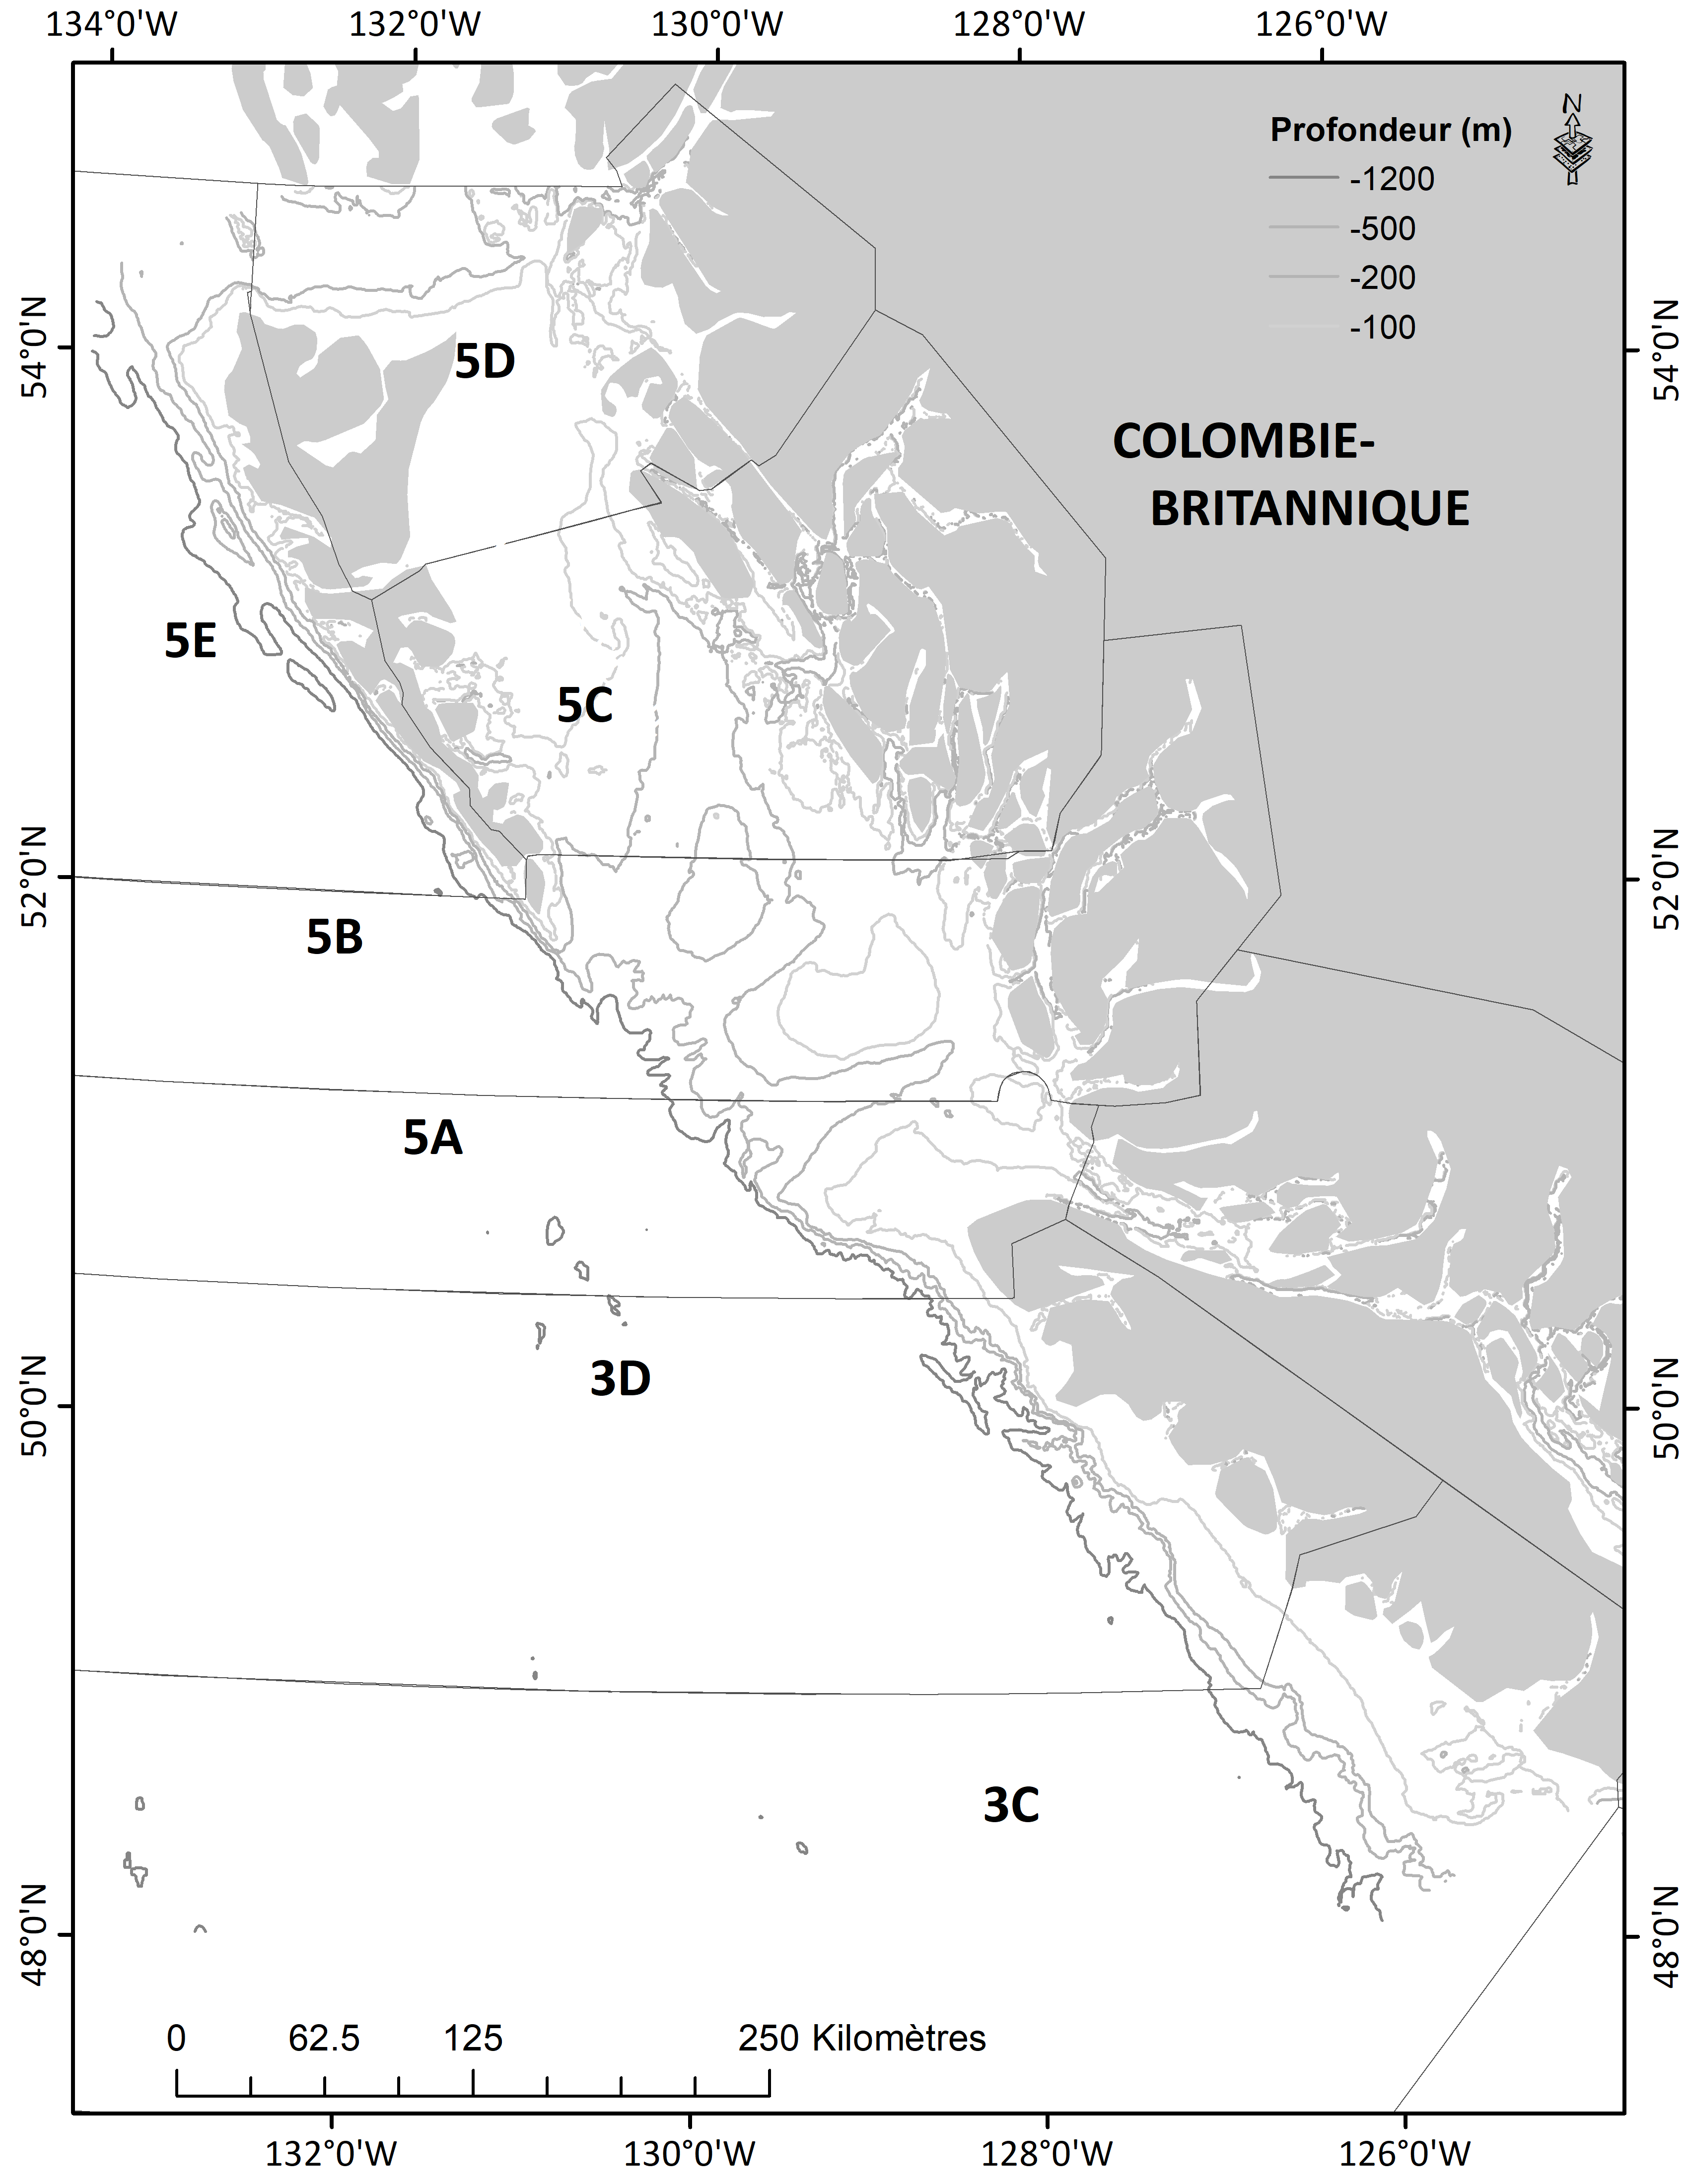
\includegraphics[width=4in]{C:/GitHub/pacific-cod-2020/report/figure/Pcod_3CD5ABCDE_Pic}}{Figure \ref{fig:fig-map}} 

}

\caption{Map of the management areas 5AB (Queen Charlotte Sound), 5CD (Hecate Strait), and 3CD (West Coast Vancouver Island).}\label{fig:fig-map}
\end{figure}
\clearpage

\hypertarget{sec:figures}{%
\subsection{CATCH: AREA 5ABCD}\label{sec:figures}}
\begin{figure}[htb]

{\centering \pdftooltip{\includegraphics[width=6in]{knitr-figs/fig-catch-5abcd-1}}{Figure \ref{fig:fig-catch-5abcd}} 

}

\caption{Catch for Area 5ABCD. Canadian catch includes at-sea releases.}\label{fig:fig-catch-5abcd}
\end{figure}
\begin{figure}[htb]

{\centering \pdftooltip{\includegraphics[width=6in]{knitr-figs/fig-discards-5abcd-1}}{Figure \ref{fig:fig-discards-5abcd}} 

}

\caption{Estimated at-sea releases of Pacific Cod by bottom trawlers for Area 5ABCD.}\label{fig:fig-discards-5abcd}
\end{figure}
\begin{figure}[htb]

{\centering \pdftooltip{\includegraphics[width=6in]{knitr-figs/fig-catch-5ab-1}}{Figure \ref{fig:fig-catch-5ab}} 

}

\caption{Catch for Area 5AB. Canadian catch includes at-sea releases.}\label{fig:fig-catch-5ab}
\end{figure}
\begin{figure}[htb]

{\centering \pdftooltip{\includegraphics[width=6in]{knitr-figs/fig-discards-5ab-1}}{Figure \ref{fig:fig-discards-5ab}} 

}

\caption{Estimated at-sea releases of Pacific Cod by bottom trawlers for Area 5AB.}\label{fig:fig-discards-5ab}
\end{figure}
\begin{figure}[htb]

{\centering \pdftooltip{\includegraphics[width=6in]{knitr-figs/fig-catch-5cd-1}}{Figure \ref{fig:fig-catch-5cd}} 

}

\caption{Catch for Area 5CD. Canadian catch includes at-sea releases.}\label{fig:fig-catch-5cd}
\end{figure}
\begin{figure}[htb]

{\centering \pdftooltip{\includegraphics[width=6in]{knitr-figs/fig-discards-5cd-1}}{Figure \ref{fig:fig-discards-5cd}} 

}

\caption{Estimated at-sea releases of Pacific Cod by bottom trawlers for Area 5CD.}\label{fig:fig-discards-5cd}
\end{figure}
\clearpage

\hypertarget{catch-area-3cd}{%
\subsection{CATCH: AREA 3CD}\label{catch-area-3cd}}
\begin{figure}[htb]

{\centering \pdftooltip{\includegraphics[width=6in]{knitr-figs/fig-catch-3cd-1}}{Figure \ref{fig:fig-catch-3cd}} 

}

\caption{Catch for Area 3CD. Canadian catch includes at-sea releases.}\label{fig:fig-catch-3cd}
\end{figure}
\begin{figure}[htb]

{\centering \pdftooltip{\includegraphics[width=6in]{knitr-figs/fig-discards-3cd-1}}{Figure \ref{fig:fig-discards-3cd}} 

}

\caption{Estimated at-sea releases of Pacific Cod by bottom trawlers for Area 3CD.}\label{fig:fig-discards-3cd}
\end{figure}
\clearpage

\hypertarget{prior-probability-distributions}{%
\subsection{PRIOR PROBABILITY DISTRIBUTIONS}\label{prior-probability-distributions}}
\begin{figure}[htb]

{\centering \pdftooltip{\includegraphics[width=6in]{knitr-figs/fig-base-mcmc-priors-5abcd-1}}{Figure \ref{fig:fig-base-mcmc-priors-5abcd}} 

}

\caption{Prior probability distributions used in the Area 5ABCD reference model. $q_1$ = Hecate Strait Assemblage survey, $q_2$ = Queen Charlotte Sound Synoptic Survey, $q_3$ = Hecate Strait Synoptic Survey, $q_4$ = Commercial CPUE pre-1996, and $q_5$ = Commercial CPUE post-1995.}\label{fig:fig-base-mcmc-priors-5abcd}
\end{figure}
\begin{figure}[htb]

{\centering \pdftooltip{\includegraphics[width=6in]{knitr-figs/fig-base-mcmc-priors-3cd-1}}{Figure \ref{fig:fig-base-mcmc-priors-3cd}} 

}

\caption{Prior probability distributions used in the Area 3CD reference model. $q_1$ = West Coast Vancouver Island Synoptic Survey, $q_2$ = Commercial CPUE pre-1996, $q_3$ = Commercial CPUE post-1995, and $q_4$ = NMFS Triennial Survey (Canadian portion).}\label{fig:fig-base-mcmc-priors-3cd}
\end{figure}
\clearpage

\hypertarget{model-results-area-5abcd}{%
\subsection{MODEL RESULTS: AREA 5ABCD}\label{model-results-area-5abcd}}
\begin{figure}[htb]

{\centering \pdftooltip{\includegraphics[width=6in]{knitr-figs/fig-base-mcmc-trace-5abcd-1}}{Figure \ref{fig:fig-base-mcmc-trace-5abcd}} 

}

\caption{Traceplots of posterior samples for the Area 5ABCD reference model. $q_1$ = Hecate Strait Assemblage survey, $q_2$ = Queen Charlotte Sound Synoptic Survey, $q_3$ = Hecate Strait Synoptic Survey, $q_4$ = Commercial CPUE pre-1996, and $q_5$ = Commercial CPUE post-1995.}\label{fig:fig-base-mcmc-trace-5abcd}
\end{figure}
\begin{figure}[htb]

{\centering \pdftooltip{\includegraphics[width=6in]{knitr-figs/fig-base-mcmc-autocor-5abcd-1}}{Figure \ref{fig:fig-base-mcmc-autocor-5abcd}} 

}

\caption{Autocorrelation plots for the Area 5ABCD reference model. $q_1$ = Hecate Strait Assemblage survey, $q_2$ = Queen Charlotte Sound Synoptic Survey, $q_3$ = Hecate Strait Synoptic Survey, $q_4$ = Commercial CPUE pre-1996, and $q_5$ = Commercial CPUE post-1995.}\label{fig:fig-base-mcmc-autocor-5abcd}
\end{figure}
\begin{figure}[htb]

{\centering \pdftooltip{\includegraphics[width=6in]{knitr-figs/fig-base-index-fits-5abcd-1}}{Figure \ref{fig:fig-base-index-fits-5abcd}} 

}

\caption{MPD fits to observed indices of abundance (points) for the Area 5ABCD reference model from: (a) the Hecate Strait Assemblage survey, (b) the Queen Charlotte Sound Synoptic Survey, (c) the Hecate Strait Synoptic Survey, (d) the Commercial CPUE pre-1996, and (e) the Commercial CPUE post-1995. For clarity, only MPD results are shown}\label{fig:fig-base-index-fits-5abcd}
\end{figure}
\begin{figure}[htb]

{\centering \pdftooltip{\includegraphics[width=6in]{knitr-figs/fig-base-mean-weight-5abcd-1}}{Figure \ref{fig:fig-base-mean-weight-5abcd}} 

}

\caption{MPD fit to the mean weight data for Area 5ABCD reference model. For clarity, only MPD results are shown}\label{fig:fig-base-mean-weight-5abcd}
\end{figure}
\begin{figure}[htb]

{\centering \pdftooltip{\includegraphics[width=6in]{knitr-figs/fig-base-catch-fit-5abcd-1}}{Figure \ref{fig:fig-base-catch-fit-5abcd}} 

}

\caption{MPD fit to the catch data for Area 5ABCD reference model. For clarity, only MPD results are shown}\label{fig:fig-base-catch-fit-5abcd}
\end{figure}

\begin{figure}[htb]

{\centering \pdftooltip{\includegraphics[width=6in]{knitr-figs/fig-base-mcmc-priors-posts-5abcd-1}}{Figure \ref{fig:fig-base-mcmc-priors-posts-5abcd}} 

}

\caption{Histograms of posterior samples with prior probability distributions (lines) used in the Area 5ABCD reference model. MPD estimate shown as vertical dashed line. Note that both the Queen Charlotte Sound and Hecate Strait Synoptic Surveys used normal prior distributions on \(ln(q)\), see Figure~\ref{fig:fig-base-mcmc-priors-5abcd} for full distribution. $q_1$ = Hecate Strait Assemblage survey, $q_2$ = Queen Charlotte Sound Synoptic Survey, $q_3$ = Hecate Strait Synoptic Survey, $q_4$ = Commercial CPUE pre-1996, and $q_5$ = Commercial CPUE post-1995.}\label{fig:fig-base-mcmc-priors-posts-5abcd}
\end{figure}
\begin{figure}[htb]

{\centering \pdftooltip{\includegraphics[width=6in]{knitr-figs/fig-base-mcmc-pairs-5abcd-1}}{Figure \ref{fig:fig-base-mcmc-pairs-5abcd}} 

}

\caption{Pairs plots of posterior samples for the Area 5ABCD reference model. $\bar{R} = R_{Avg}$, $q_1$ = Hecate Strait Assemblage survey, $q_2$ = Queen Charlotte Sound Synoptic Survey, $q_3$ = Hecate Strait Synoptic Survey, $q_4$ = Commercial CPUE pre-1996, and $q_5$ = Commercial CPUE post-1995.}\label{fig:fig-base-mcmc-pairs-5abcd}
\end{figure}
\begin{figure}[htb]

{\centering \pdftooltip{\includegraphics[width=6in]{knitr-figs/fig-base-biomass-5abcd-1}}{Figure \ref{fig:fig-base-biomass-5abcd}} 

}

\caption{Posterior estimated biomass for the Reference Model, Area 5ABCD.  The green dashed line shows the median Upper Stock Reference (USR) which is the mean biomass estimate for the years 1956--2004. The red dashed line shows the median Limit Reference Point (LRP) which is the lowest estimated biomass agreed to be an undesirable state to avoid, in this case it is the biomass estimate for 2000.}\label{fig:fig-base-biomass-5abcd}
\end{figure}
\begin{figure}[htb]

{\centering \pdftooltip{\includegraphics[width=6in]{knitr-figs/fig-base-depl-5abcd-1}}{Figure \ref{fig:fig-base-depl-5abcd}} 

}

\caption{Relative biomass for the Reference Model, Area 5ABCD.}\label{fig:fig-base-depl-5abcd}
\end{figure}
\begin{figure}[htb]

{\centering \pdftooltip{\includegraphics[width=6in]{knitr-figs/fig-base-recr-5abcd-1}}{Figure \ref{fig:fig-base-recr-5abcd}} 

}

\caption{Recruitment (a) and recruitment deviations (b) for the Reference Model, Area 5ABCD.  The green dashed line shows the mean of the MCMC posterior medians, the blue dashed line shows the median of the MCMC posterior medians.}\label{fig:fig-base-recr-5abcd}
\end{figure}
\begin{figure}[htb]

{\centering \pdftooltip{\includegraphics[width=6in]{knitr-figs/fig-base-f-5abcd-1}}{Figure \ref{fig:fig-base-f-5abcd}} 

}

\caption{Fishing mortality for the Reference Model, Area 5ABCD.}\label{fig:fig-base-f-5abcd}
\end{figure}
\clearpage

\hypertarget{model-results-area-3cd}{%
\subsection{MODEL RESULTS: AREA 3CD}\label{model-results-area-3cd}}
\begin{figure}[htb]

{\centering \pdftooltip{\includegraphics[width=6in]{knitr-figs/fig-base-mcmc-trace-3cd-1}}{Figure \ref{fig:fig-base-mcmc-trace-3cd}} 

}

\caption{Traceplots of posterior samples for the Area 3CD reference model. $q_1$ = West Coast Vancouver Island Synoptic Survey, $q_2$ = Commercial CPUE pre-1996, $q_3$ = Commercial CPUE post-1995, and $q_4$ = NMFS Triennial Survey (Canadian portion).}\label{fig:fig-base-mcmc-trace-3cd}
\end{figure}
\begin{figure}[htb]

{\centering \pdftooltip{\includegraphics[width=6in]{knitr-figs/fig-base-mcmc-autocor-3cd-1}}{Figure \ref{fig:fig-base-mcmc-autocor-3cd}} 

}

\caption{Autocorrelation plots for the Area 3CD reference model. $q_1$ = West Coast Vancouver Island Synoptic Survey, $q_2$ = Commercial CPUE pre-1996, $q_3$ = Commercial CPUE post-1995, and $q_4$ = NMFS Triennial Survey (Canadian portion).}\label{fig:fig-base-mcmc-autocor-3cd}
\end{figure}
\begin{figure}[htb]

{\centering \pdftooltip{\includegraphics[width=6in]{knitr-figs/fig-base-index-fits-3cd-1}}{Figure \ref{fig:fig-base-index-fits-3cd}} 

}

\caption{MPD fits to observed indices of abundance (points) for the Area 3CD reference model from: (a) the West Coast Vancouver Island Synoptic Survey, (b) the Commercial CPUE pre-1996, (c) the Commercial CPUE post-1995, and (d) the NMFS Triennial Survey (Canadian portion).}\label{fig:fig-base-index-fits-3cd}
\end{figure}
\begin{figure}[htb]

{\centering \pdftooltip{\includegraphics[width=6in]{knitr-figs/fig-base-mean-weight-3cd-1}}{Figure \ref{fig:fig-base-mean-weight-3cd}} 

}

\caption{MPD fit to the mean weight data for Area 3CD reference model.}\label{fig:fig-base-mean-weight-3cd}
\end{figure}
\begin{figure}[htb]

{\centering \pdftooltip{\includegraphics[width=6in]{knitr-figs/fig-base-catch-fit-3cd-1}}{Figure \ref{fig:fig-base-catch-fit-3cd}} 

}

\caption{MPD fit to the catch data for Area 3CD reference model.}\label{fig:fig-base-catch-fit-3cd}
\end{figure}

\begin{figure}[htb]

{\centering \pdftooltip{\includegraphics[width=6in]{knitr-figs/fig-base-mcmc-priors-posts-3cd-1}}{Figure \ref{fig:fig-base-mcmc-priors-posts-3cd}} 

}

\caption{Histograms of posterior samples with prior probability distributions (lines) used in the Area 3CD reference model. MPD estimate shown as vertical dashed line. Note that the West Coast Vancouver Island Synoptic Survey used a normal prior distribution on \(ln(q)\), see Figure~\ref{fig:fig-base-mcmc-priors-3cd} for full distribution. $q_1$ = West Coast Vancouver Island Synoptic Survey, $q_2$ = Commercial CPUE pre-1996, $q_3$ = Commercial CPUE post-1995, and $q_4$ = NMFS Triennial Survey (Canadian portion).}\label{fig:fig-base-mcmc-priors-posts-3cd}
\end{figure}
\begin{figure}[htb]

{\centering \pdftooltip{\includegraphics[width=6in]{knitr-figs/fig-base-mcmc-pairs-3cd-1}}{Figure \ref{fig:fig-base-mcmc-pairs-3cd}} 

}

\caption{Pairs plots of posterior samples for the Area 3CD reference model. $q_1$ = West Coast Vancouver Island Synoptic Survey, $q_2$ = Commercial CPUE pre-1996, $q_3$ = Commercial CPUE post-1995, and $q_4$ = NMFS Triennial Survey (Canadian portion).}\label{fig:fig-base-mcmc-pairs-3cd}
\end{figure}
\begin{figure}[htb]

{\centering \pdftooltip{\includegraphics[width=6in]{knitr-figs/fig-base-biomass-3cd-1}}{Figure \ref{fig:fig-base-biomass-3cd}} 

}

\caption{Posterior estimated biomass for the Reference Model, Area 3CD. The green dashed line shows the median Upper Stock Reference (USR) which is the mean biomass estimate for the years 1956--2004. The red dashed line shows the median Limit Reference Point (LRP) which is the lowest estimated biomass agreed to be an undesirable state to avoid, in this case it is the biomass estimate for 1986.}\label{fig:fig-base-biomass-3cd}
\end{figure}
\begin{figure}[htb]

{\centering \pdftooltip{\includegraphics[width=6in]{knitr-figs/fig-base-depl-3cd-1}}{Figure \ref{fig:fig-base-depl-3cd}} 

}

\caption{Relative biomass for the Reference Model, Area 3CD.}\label{fig:fig-base-depl-3cd}
\end{figure}
\begin{figure}[htb]

{\centering \pdftooltip{\includegraphics[width=6in]{knitr-figs/fig-base-recr-3cd-1}}{Figure \ref{fig:fig-base-recr-3cd}} 

}

\caption{Recruitment (a) and recruitment deviations (b) for the Reference Model, Area 3CD.  The green dashed line shows the mean of the MCMC posterior medians, the blue dashed line shows the median of the MCMC posterior medians.}\label{fig:fig-base-recr-3cd}
\end{figure}
\begin{figure}[htb]

{\centering \pdftooltip{\includegraphics[width=6in]{knitr-figs/fig-base-f-3cd-1}}{Figure \ref{fig:fig-base-f-3cd}} 

}

\caption{Fishing mortality for the Reference Model, Area 3CD.}\label{fig:fig-base-f-3cd}
\end{figure}
\clearpage
\begin{figure}[htb]

{\centering \pdftooltip{\includegraphics[width=6in]{knitr-figs/fig-model-average-biomass-comp-5abcd-1}}{Figure \ref{fig:fig-model-average-biomass-comp-5abcd}} 

}

\caption{Posterior estimates of biomass for the model-averaged set for Area 5ABCD. The green dashed line shows the median Upper Stock Reference (USR) which is the mean biomass estimate for the years 1956--2004. The red dashed line shows the median Limit Reference Point (LRP) which is the lowest estimated biomass agreed to be an undesirable state to avoid, in this case it is the biomass estimate for 2000.}\label{fig:fig-model-average-biomass-comp-5abcd}
\end{figure}
\begin{figure}[htb]

{\centering \pdftooltip{\includegraphics[width=6in]{knitr-figs/fig-model-average-biomass-5abcd-1}}{Figure \ref{fig:fig-model-average-biomass-5abcd}} 

}

\caption{Combined posterior biomass for the averaged models, Area 5ABCD. The green dashed line shows the median Upper Stock Reference (USR) which is the mean biomass estimate for the years 1956--2004. The red dashed line shows the median Limit Reference Point (LRP) which is the lowest estimated biomass agreed to be an undesirable state to avoid, in this case it is the biomass estimate for 2000.}\label{fig:fig-model-average-biomass-5abcd}
\end{figure}
\clearpage
\begin{figure}[htb]

{\centering \pdftooltip{\includegraphics[width=6in]{knitr-figs/fig-model-average-biomass-5abcd-proj-1}}{Figure \ref{fig:fig-model-average-biomass-5abcd-proj}} 

}

\caption{Combined posterior estimates of biomass for the model-averaged set for Area 5ABCD with projections (to the end of 2019).  The upper horizontal green dashed line shows the median Upper Stock Reference (USR) which is the mean biomass estimate for the years 1956--2004. The lower horizontal red dashed line shows the median Limit Reference Point (LRP) which is the lowest estimated biomass agreed to be an undesirable state to avoid, in this case it is the biomass estimate for 2000. The coloured regions to the right of the vertical line represent projections based on various TACs. The line represents the posterior median and the shaded region represents the 95\% credible interval. For clarity, years before 2010 are removed.}\label{fig:fig-model-average-biomass-5abcd-proj}
\end{figure}
\clearpage
\begin{figure}[htb]

{\centering \pdftooltip{\includegraphics[width=6in]{knitr-figs/fig-model-average-biomass-comp-3cd-1}}{Figure \ref{fig:fig-model-average-biomass-comp-3cd}} 

}

\caption{Posterior estimates of biomass for the model-averaged set for Area 3CD. The green dashed line shows the median Upper Stock Reference (USR) which is the mean biomass estimate for the years 1956--2004. The red dashed line shows the median Limit Reference Point (LRP) which is the lowest estimated biomass agreed to be an undesirable state to avoid, in this case it is the biomass estimate for 1986.}\label{fig:fig-model-average-biomass-comp-3cd}
\end{figure}
\clearpage
\begin{figure}[htb]

{\centering \pdftooltip{\includegraphics[width=6in]{knitr-figs/fig-model-average-biomass-3cd-1}}{Figure \ref{fig:fig-model-average-biomass-3cd}} 

}

\caption{Combined posterior biomass for the model-averaged set for Area 3CD.  The green dashed line shows the median Upper Stock Reference (USR) which is the mean biomass estimate for the years 1956--2004. The red dashed line shows the median Limit Reference Point (LRP) which is the lowest estimated biomass agreed to be an undesirable state to avoid, in this case it is the biomass estimate for 1986.}\label{fig:fig-model-average-biomass-3cd}
\end{figure}
\clearpage
\begin{figure}[htb]

{\centering \pdftooltip{\includegraphics[width=6in]{knitr-figs/fig-model-average-biomass-3cd-proj-1}}{Figure \ref{fig:fig-model-average-biomass-3cd-proj}} 

}

\caption{Combined posterior estimates of biomass for the model-averaged set for Area 3CD with projections (to the end of 2019).  The upper horizontal green dashed line shows the median Upper Stock Reference (USR) which is the mean biomass estimate for the years 1956--2004. The lower horizontal red dashed line shows the median Limit Reference Point (LRP) which is the lowest estimated biomass agreed to be an undesirable state to avoid, in this case it is the biomass estimate for 2000. The coloured regions to the right of the vertical line represent projections based on various TACs. The line represents the posterior median and the shaded region represents the 95\% credible interval.For clarity, years before 2010 are removed.}\label{fig:fig-model-average-biomass-3cd-proj}
\end{figure}
\clearpage

\Appendices


\clearpage

\refstepcounter{chapter}
\label{app:survey-appendix}
\starredchapter{APPENDIX~\thechapter. FISHERY-INDEPENDENT INDICES OF ABUNDANCE}

\hypertarget{canadian-surveys}{%
\appsection{CANADIAN SURVEYS}\label{canadian-surveys}}

\hypertarget{hecate-strait-assemblage-survey}{%
\subsection{HECATE STRAIT ASSEMBLAGE SURVEY}\label{hecate-strait-assemblage-survey}}

A series of multi-species groundfish bottom trawl surveys was conducted in Hecate Strait in May-June of 1984, 1987, 1989, 1991, 1993, 1995, 1996, 1998, 2000, 2002, and 2003 Westrheim et al. (\protect\hyperlink{ref-westrheim1984}{1984}), Fargo et al. (\protect\hyperlink{ref-fargo1984}{1984}), Fargo et al. (\protect\hyperlink{ref-fargo1988}{1988}), Wilson et al. (\protect\hyperlink{ref-wilson1991}{1991}), Hand et al. (\protect\hyperlink{ref-hand1994}{1994}), Workman et al. (\protect\hyperlink{ref-workman1996}{1996}), Workman et al. (\protect\hyperlink{ref-workman1997}{1997}), Choromanski et al. (\protect\hyperlink{ref-choromanski2002}{2002})) (Figure~\ref{fig:survey-maps-hs-msa}. The results up to 2000 were reported in the 2001 assessment (Sinclair et al. \protect\hyperlink{ref-sinclair2001}{2001}) and results from 2002 and 2003 were presented in the 2005 assessment (Sinclair and Starr \protect\hyperlink{ref-sinclair2005}{2005}).

The original design of this survey assigned fishing locations by 10 fm depth intervals within a 10 nm grid of Hecate Strait. The survey was post-stratified for the purpose of calculating an abundance index for Pacific Cod (Sinclair \protect\hyperlink{ref-sinclair2000}{1999}). The post stratification used 10 fm depth intervals for the entire survey area, thereby treating each depth interval as a single stratum.

The Hecate Strait Assemblage survey was designed as a systematic fixed-station survey. Despite attempts to apply post-sampling stratification, this approach had high survey variance (Sinclair et al. \protect\hyperlink{ref-sinclair2007}{2007}). In 2004 the Hecate Strait Assemblage survey was discontinued in favour of the Hecate Strait Synoptic survey (described below).

\hypertarget{hecate-strait-synoptic-survey}{%
\subsection{HECATE STRAIT SYNOPTIC SURVEY}\label{hecate-strait-synoptic-survey}}

The Hecate Strait synoptic groundfish bottom trawl survey is part of a coordinated set of long-term surveys that together cover the continental shelf and upper slope of most of the BC coast (Figure~\ref{fig:survey-maps-syn-hs}. The Hecate Strait synoptic survey has been conducted during May-June, in odd years since 2005. All the synoptic surveys follow a random depth stratified design. The survey area is divided into 2 km by 2 km blocks and each block is assigned to one of four depth strata based on the average bottom depth in the block. The four depth strata for the Hecate Strait survey are 10--70m, 70--130m, 130--220m, and 220--500m. Each year blocks are randomly selected within each depth strata. For this survey and the other synoptic surveys discussed below, the relative allocation of blocks amongst depth strata was determined by modeling the expected catches of groundfish and determining the target number of tows per stratum that would provide sufficiently precise catch rate data for as many species as possible.

\hypertarget{queen-charlotte-sound-synoptic-survey}{%
\subsection{QUEEN CHARLOTTE SOUND SYNOPTIC SURVEY}\label{queen-charlotte-sound-synoptic-survey}}

The Queen Charlotte Sound (QCS) synoptic groundfish bottom trawl survey has been conducted in July--August in 2003, 2004, and in odd years since 2005 (Figure~\ref{fig:survey-maps-syn-qcs}. The four depth strata for the QCS survey are 50--125m, 125--200m, 200--330m, and 330--500 m. Each year blocks are randomly selected within each depth strata. In addition, for the purposes of allocating blocks, the QCS survey is divided into northern and southern spatial strata.

\hypertarget{west-coast-vancouver-island-synoptic-survey}{%
\subsection{WEST COAST VANCOUVER ISLAND SYNOPTIC SURVEY}\label{west-coast-vancouver-island-synoptic-survey}}

The West Coast Vancouver Island synoptic bottom trawl survey was first conducted in 2004 and is conducted in alternating (even-numbered) years on a chartered commercial trawler (Figure~\ref{fig:survey-maps-syn-wcvi}). The survey area is off the west coast of Vancouver Island from approximately 49 \(^\circ\) 12\(^\prime\) to 50 \(^\circ\) 36\(^\prime\) North latitude and approximately 124 \(^\circ\) 48\(^\prime\) to 128 \(^\circ\) 30\(^\prime\) West longitude. The southern boundary is contiguous with the Canada/U.S. boundary. The survey has a single aerial stratum in Pacific Fishery Management Area regions 3C and 3D separated into four depth strata: 50--125m; 125--200m; 200--330m; and 330--500m. Approximately 150 to 180 4 km\textsuperscript{2} blocks are selected randomly among the four depth strata when conducting each survey.
\begin{figure}[htb]

{\centering \pdftooltip{\includegraphics[width=6in]{knitr-figs/survey-maps-hs-msa-1}}{Figure \ref{fig:survey-maps-hs-msa}} 

}

\caption{Individual survey tows for the Hecate Strait multi-species groundfish bottom trawl survey. Light gray crosses indicate survey sets that did not catch Pacific Cod. Circles have their area and color proportional to the density of Pacific Cod for that survey set. Eastings and Northings are for UTM zone 9.}\label{fig:survey-maps-hs-msa}
\end{figure}
\begin{figure}[htb]

{\centering \pdftooltip{\includegraphics[width=6in]{knitr-figs/survey-maps-syn-hs-1}}{Figure \ref{fig:survey-maps-syn-hs}} 

}

\caption{Individual survey tows for the Hecate Strait (SYN HS) synoptic groundfish bottom trawl survey. Light gray crosses indicate survey sets that did not catch Pacific Cod. Circles have their area and color proportional to the density of Pacific Cod for that survey set. Eastings and Northings are for UTM zone 9.}\label{fig:survey-maps-syn-hs}
\end{figure}
\begin{figure}[htb]

{\centering \pdftooltip{\includegraphics[width=6in]{knitr-figs/survey-maps-syn-qcs-1}}{Figure \ref{fig:survey-maps-syn-qcs}} 

}

\caption{Individual survey tows for the Queen Charlotte Sound (SYN QCS) synoptic groundfish bottom trawl survey. Light gray crosses indicate survey sets that did not catch Pacific Cod. Circles have their area and color proportional to the density of Pacific Cod for that survey set. Eastings and Northings are for UTM zone 9.}\label{fig:survey-maps-syn-qcs}
\end{figure}
\begin{figure}[htb]

{\centering \pdftooltip{\includegraphics[width=6in]{knitr-figs/survey-maps-syn-wcvi-1}}{Figure \ref{fig:survey-maps-syn-wcvi}} 

}

\caption{Individual survey tows for the West Coast Vancouver Island (SYN WCVI) synoptic groundfish bottom trawl survey survey. Light gray crosses indicate survey sets that did not catch Pacific Cod. Circles have their area and color proportional to the density of Pacific Cod for that survey set. Eastings and Northings are for UTM zone 9.}\label{fig:survey-maps-syn-wcvi}
\end{figure}
\clearpage

\hypertarget{swept-area-analysis}{%
\subsection{SWEPT AREA ANALYSIS}\label{swept-area-analysis}}

For all Canadian surveys, a swept area estimate of biomass in any year \(y\) was obtained by summing the product of the CPUE and the area surveyed across the surveyed strata \(i\):
\begin{equation}
  B_y = \sum_{i=1}^kC_{y_i}A_i=\sum_{i=1}^kB_{y_i}
  \label{eq:sweptareabiomass}
\end{equation}
where \(C_{y_i}\) = mean CPUE density (kg/km\textsuperscript{2}) for Pacific Cod in stratum \(i\), \(A_i\) = area of stratum \(i\) (km\textsuperscript{2}), \(B_{y_i}\) = biomass of Pacific Cod in stratum \(i\) for year \(y\), and \(k\) = number of strata.

CPUE (\(C_{y_i}\)) for Pacific Cod in stratum \(i\) for year \(y\) was calculated as a density in kg/km\textsuperscript{2} by
\begin{equation}
  C_{y_i}=\frac{1}{n_{y_i}} \sum\limits_{j=1}^{n_{y_i}} \frac{W_{y_i,j}}{D_{y_i,j}w_{y_i,j}}
  \label{eq:sweptareacpue}
\end{equation}
where \(W_{y_i,j}\) = catch weight (kg) for Pacific Cod in stratum \(i\) for year \(y\) and tow \(j\), \(D_{y_i,j}\) = distance travelled (km) by tow \(j\) in stratum \(i\) for year \(y\), \(w_{y_i,j}\) = net opening (km) by tow \(j\) in stratum \(i\) for year \(y\), and \(n_{y_i}\) = number of tows in stratum \(i\).

The variance of the survey biomass estimate \(V_y\) for Pacific Cod in year \(y\) was calculated in kg\textsuperscript{2} as follows:
\begin{equation}
  V_y=\sum_{i=1}^k\frac{\sigma_{y_i}^2A_i^2}{n_{y_i}}=\sum_{i=1}^kV_{y_i}
  \label{eq:sweptareavariance}
\end{equation}
where \(\sigma_{y_i}^2\) is the variance of the CPUE in \(kg^2/km^4\) for year \(y\) in stratum \(i\), \(V_{y_i}\) is the variance of Pacific Cod in stratum \(i\) for year \(y\), and where \(\sigma_{y_i}^2\) was obtained from bootstrapped samples (see below).

The CV for Pacific Cod for each year \(y\) was calculated as follows:
\begin{equation}
  (CV)_y=\frac{{V_y}^{1/2}}{B_y}
  \label{eq:sweptareacv}
\end{equation}
where \((CV)_y\) is the CV for year \(y\).

One thousand bootstrap replicates with replacement were constructed from the survey data to estimate bias corrected 95\% confidence intervals for each survey year (Efron \protect\hyperlink{ref-efron1982}{1982}). The resulting values are shown in Table~\ref{tab:surv-canadian-table} and Figure~\ref{fig:surv-canadian}.
\begin{longtable}[]{@{}lrrrrrrr@{}}
\caption{\label{tab:surv-canadian-table}Pacific Cod survey data for Canadian trawl surveys. Relative biomass and associated lower and upper confidence intervals (CI) are shown in metric tons (without accounting for survey catchability). Positive sets refers to the number of trawl sets that caught Pacific Cod.}\tabularnewline
\toprule
Survey abbrev. & Year & Biomass & CV & Lower CI & Upper CI & Sets & Positive sets\tabularnewline
\midrule
\endfirsthead
\toprule
Survey abbrev. & Year & Biomass & CV & Lower CI & Upper CI & Sets & Positive sets\tabularnewline
\midrule
\endhead
OTHER HS MSA & 1984 & 1142.4 & 0.30 & 606.6 & 1929.9 & 146 & 88\tabularnewline
OTHER HS MSA & 1987 & 3875.7 & 0.35 & 1501.2 & 6778.9 & 85 & 43\tabularnewline
OTHER HS MSA & 1989 & 4102.8 & 0.43 & 1318.5 & 7976.0 & 90 & 48\tabularnewline
OTHER HS MSA & 1991 & 1031.8 & 0.30 & 506.1 & 1679.0 & 97 & 59\tabularnewline
OTHER HS MSA & 1993 & 1255.6 & 0.24 & 719.9 & 1862.4 & 94 & 40\tabularnewline
OTHER HS MSA & 1995 & 1419.8 & 0.46 & 528.7 & 2880.5 & 101 & 52\tabularnewline
OTHER HS MSA & 1996 & 1418.5 & 0.26 & 793.2 & 2208.0 & 158 & 83\tabularnewline
OTHER HS MSA & 1998 & 4253.0 & 0.51 & 1223.7 & 9186.9 & 86 & 52\tabularnewline
OTHER HS MSA & 2000 & 436.1 & 0.20 & 283.7 & 622.8 & 105 & 54\tabularnewline
OTHER HS MSA & 2002 & 2025.9 & 0.27 & 1137.3 & 3203.6 & 91 & 66\tabularnewline
OTHER HS MSA & 2003 & 1288.7 & 0.21 & 808.3 & 1871.8 & 95 & 77\tabularnewline
SYN HS & 2005 & 1946.4 & 0.24 & 1192.6 & 2992.5 & 198 & 161\tabularnewline
SYN HS & 2007 & 586.6 & 0.22 & 359.5 & 856.2 & 132 & 72\tabularnewline
SYN HS & 2009 & 2460.8 & 0.45 & 744.7 & 4918.3 & 155 & 102\tabularnewline
SYN HS & 2011 & 1860.7 & 0.26 & 1083.4 & 2978.7 & 184 & 124\tabularnewline
SYN HS & 2013 & 2326.5 & 0.24 & 1443.3 & 3512.3 & 175 & 132\tabularnewline
SYN HS & 2015 & 956.6 & 0.21 & 598.9 & 1394.0 & 148 & 107\tabularnewline
SYN HS & 2017 & 1554.4 & 0.34 & 754.4 & 2792.0 & 138 & 107\tabularnewline
SYN HS & 2019 & 1752.1 & 0.37 & 832.3 & 3204.5 & 136 & 102\tabularnewline
SYN QCS & 2003 & 806.6 & 0.17 & 568.1 & 1092.1 & 233 & 101\tabularnewline
SYN QCS & 2004 & 1624.4 & 0.26 & 901.8 & 2550.5 & 230 & 118\tabularnewline
SYN QCS & 2005 & 1505.0 & 0.35 & 785.6 & 2705.1 & 224 & 125\tabularnewline
SYN QCS & 2007 & 434.5 & 0.25 & 245.5 & 665.9 & 255 & 105\tabularnewline
SYN QCS & 2009 & 565.5 & 0.24 & 335.1 & 859.5 & 233 & 95\tabularnewline
SYN QCS & 2011 & 1018.4 & 0.21 & 644.6 & 1473.9 & 251 & 98\tabularnewline
SYN QCS & 2013 & 928.3 & 0.15 & 680.9 & 1232.9 & 240 & 134\tabularnewline
SYN QCS & 2015 & 1122.3 & 0.29 & 644.0 & 1852.9 & 238 & 124\tabularnewline
SYN QCS & 2017 & 521.8 & 0.17 & 355.2 & 706.0 & 240 & 90\tabularnewline
SYN QCS & 2019 & 1004.0 & 0.13 & 782.6 & 1283.6 & 242 & 113\tabularnewline
SYN WCHG & 2006 & 50.7 & 0.23 & 30.6 & 75.7 & 110 & 36\tabularnewline
SYN WCHG & 2007 & 33.0 & 0.42 & 10.4 & 62.9 & 111 & 23\tabularnewline
SYN WCHG & 2008 & 12.4 & 0.27 & 6.4 & 19.8 & 118 & 20\tabularnewline
SYN WCHG & 2010 & 21.4 & 0.46 & 7.6 & 43.9 & 129 & 27\tabularnewline
SYN WCHG & 2012 & 39.8 & 0.31 & 19.8 & 68.6 & 130 & 34\tabularnewline
SYN WCHG & 2016 & 30.4 & 0.16 & 21.2 & 41.2 & 111 & 41\tabularnewline
SYN WCHG & 2018 & 20.1 & 0.25 & 11.2 & 31.3 & 119 & 22\tabularnewline
SYN WCVI & 2004 & 1133.1 & 0.22 & 696.4 & 1652.4 & 89 & 54\tabularnewline
SYN WCVI & 2006 & 1156.0 & 0.22 & 689.1 & 1693.5 & 164 & 88\tabularnewline
SYN WCVI & 2008 & 512.6 & 0.40 & 233.1 & 986.2 & 159 & 65\tabularnewline
SYN WCVI & 2010 & 1577.4 & 0.17 & 1087.3 & 2128.2 & 136 & 100\tabularnewline
SYN WCVI & 2012 & 921.3 & 0.18 & 626.2 & 1279.6 & 151 & 94\tabularnewline
SYN WCVI & 2014 & 2149.4 & 0.20 & 1342.7 & 3076.3 & 146 & 110\tabularnewline
SYN WCVI & 2016 & 2026.8 & 0.19 & 1325.7 & 2877.8 & 140 & 99\tabularnewline
SYN WCVI & 2018 & 552.9 & 0.21 & 362.3 & 805.9 & 190 & 91\tabularnewline
\bottomrule
\end{longtable}
\begin{figure}[htb]

{\centering \pdftooltip{\includegraphics[width=6in]{knitr-figs/surv-canadian-1}}{Figure \ref{fig:surv-canadian}} 

}

\caption{Pacific Cod survey data for Canadian trawl surveys. Shown is relative biomass and associated lower and upper confidence intervals. Positive sets refers to the number of trawl sets that caught Pacific Cod.}\label{fig:surv-canadian}
\end{figure}
\clearpage

\hypertarget{nmfs-triennial-survey-in-canadian-waters}{%
\appsection{NMFS TRIENNIAL SURVEY (IN CANADIAN WATERS)}\label{nmfs-triennial-survey-in-canadian-waters}}

A relative abundance index was developed for Area 3CD from data from the National Marine Fisheries Service (NMFS) Triennial survey operated off the lower half of Vancouver Island. See Appendix A of Forrest et al. (\protect\hyperlink{ref-forrest2018}{2018}) for complete details.
\begin{figure}[htb]

{\centering \pdftooltip{\includegraphics[width=6in]{C:/GitHub/pacific-cod-2020/report/paul-figs/paul9}}{Figure \ref{fig:tri-fig9}} 

}

\caption{Biomass estimates for three series of Pacific Cod in the INPFC Vancouver region (total region, Canadian waters only, US waters only) with 95\% error bars estimated from 1000 bootstraps.}\label{fig:tri-fig9}
\end{figure}
\clearpage

\clearpage


\clearpage

\refstepcounter{chapter}
\label{app:cpue-appendix}
\starredchapter{APPENDIX~\thechapter. COMMERCIAL CPUE STANDARDIZATION}

We used the same approach for standardizing the historical (1956:1995) and modern (1996+) commercial CPUE indices as in the previous assessment (Forrest et al. \protect\hyperlink{ref-forrest2020}{2020}), with data added for 2018 and 2019.

\emph{TODO: Put some 2018 text back}
\begin{figure}[htb]

{\centering \pdftooltip{\includegraphics[width=6in]{knitr-figs/cpue-locality-map-5-1}}{Figure \ref{fig:cpue-locality-map-5}} 

}

\caption{DFO localities used in the 5ABCD modern CPUE standardization model.}\label{fig:cpue-locality-map-5}
\end{figure}
\begin{figure}[htb]

{\centering \pdftooltip{\includegraphics[width=6in]{knitr-figs/cpue-locality-map-3-1}}{Figure \ref{fig:cpue-locality-map-3}} 

}

\caption{DFO localities used in the 3CD modern CPUE standardization model.}\label{fig:cpue-locality-map-3}
\end{figure}
\begin{figure}[htb]

{\centering \pdftooltip{\includegraphics[width=6in]{knitr-figs/cpue-tweedie-ex-1}}{Figure \ref{fig:cpue-tweedie-ex}} 

}

\caption{Example density functions for the Tweedie distribution. The symbol $\phi$ (written as phi in this figure) represents the dispersion parameter, $p$ represents the power parameter, and $\mu$ represents the mean. Note that the spike in density that is seen towards the left of the panels is at a value of 0 on the x axis.}\label{fig:cpue-tweedie-ex}
\end{figure}
\begin{figure}[htb]

{\centering \pdftooltip{\includegraphics[width=6in]{knitr-figs/cpue-catch-effort-ts-1}}{Figure \ref{fig:cpue-catch-effort-ts}} 

}

\caption{Raw time series of Pacific Cod catch and total hours trawled (regardless of species caught). Data prior to 1996 is shown separately from data after 1996.}\label{fig:cpue-catch-effort-ts}
\end{figure}
\begin{figure}[htb]

{\centering \pdftooltip{\includegraphics[width=6in]{knitr-figs/cpue-depth-hists-1}}{Figure \ref{fig:cpue-depth-hists}} 

}

\caption{The depth distribution for fishing trips (top row) and fishing trawl events (bottom row) that caught Pacific Cod or did not catch Pacific Cod.}\label{fig:cpue-depth-hists}
\end{figure}
\begin{figure}[htb]

{\centering \pdftooltip{\includegraphics[width=6in]{knitr-figs/cpue-bubble-plots-hist-3CD-1}}{Figure \ref{fig:cpue-bubble-plots-hist-3CD}} 

}

\caption{Distribution of predictors in CPUE standardization models for 1956--1995 3CD dataset. Area of outermost circles represents the number of trip-locality combinations for that predictor value and year combination. Area and shading of innermost circles represents the number of trip-locality combinations for that predictor value and year combination that caught Pacific Cod.}\label{fig:cpue-bubble-plots-hist-3CD}
\end{figure}

\begin{figure}[htb]

{\centering \pdftooltip{\includegraphics[width=6in]{knitr-figs/cpue-bubble-plots-hist-5ABCD-1}}{Figure \ref{fig:cpue-bubble-plots-hist-5ABCD}} 

}

\caption{Same as Figure~\ref{fig:cpue-bubble-plots-hist-3CD} but for 5ABCD. (ref:caption-cpue-bubble-plots-modern-3CD) Same as Figure~\ref{fig:cpue-bubble-plots-hist-3CD} but for 1996--2017 3CD. (ref:caption-cpue-bubble-plots-modern-5ABCD) Same as Figure~\ref{fig:cpue-bubble-plots-hist-3CD} but for 1996--2017 5ABCD.}\label{fig:cpue-bubble-plots-hist-5ABCD}
\end{figure}
\begin{figure}[htb]

{\centering \pdftooltip{\includegraphics[width=6in]{knitr-figs/cpue-bubble-plots-modern-3CD-1}}{Figure \ref{fig:cpue-bubble-plots-modern-3CD}} 

}

\caption{(ref:caption-cpue-bubble-plots-modern-3CD)}\label{fig:cpue-bubble-plots-modern-3CD}
\end{figure}
\begin{figure}[htb]

{\centering \pdftooltip{\includegraphics[width=6in]{knitr-figs/cpue-bubble-plots-modern-5ABCD-1}}{Figure \ref{fig:cpue-bubble-plots-modern-5ABCD}} 

}

\caption{(ref:caption-cpue-bubble-plots-modern-5ABCD)}\label{fig:cpue-bubble-plots-modern-5ABCD}
\end{figure}

\begin{figure}[htb]

{\centering \pdftooltip{\includegraphics[width=6in]{knitr-figs/cpue-quantile-residuals-1}}{Figure \ref{fig:cpue-quantile-residuals}} 

}

\caption{Histograms of randomized quantile residuals (Dunn and Smyth \protect\hyperlink{ref-dunn1996}{1996}) for the CPUE GLMM standardization models. The histograms illustrate the actual density distribution of 10,000 randomly selected randomized quantile residuals. The dashed lines show the probability density for a normal distribution with the same standard deviation.}\label{fig:cpue-quantile-residuals}
\end{figure}
\begin{longtable}[]{@{}llr@{}}
\caption{\label{tab:cpue-pars}Random effect standard deviation (SD) and Tweedie observation model power (\(p\)) and dispersion (\(\phi\)) parameter estimates.}\tabularnewline
\toprule
Model & Parameter & Estimate\tabularnewline
\midrule
\endfirsthead
\toprule
Model & Parameter & Estimate\tabularnewline
\midrule
\endhead
Historical 3CD & locality SD & 0.83\tabularnewline
Historical 3CD & year-locality SD & 0.83\tabularnewline
Historical 3CD & \(p\) & 1.58\tabularnewline
Historical 3CD & \(\phi\) & 17.97\tabularnewline
Historical 5ABCD & locality SD & 0.82\tabularnewline
Historical 5ABCD & year-locality SD & 0.79\tabularnewline
Historical 5ABCD & \(p\) & 1.61\tabularnewline
Historical 5ABCD & \(\phi\) & 16.22\tabularnewline
Modern 3CD & locality SD & 0.44\tabularnewline
Modern 3CD & vessel SD & 0.19\tabularnewline
Modern 3CD & year-locality SD & 0.66\tabularnewline
Modern 3CD & \(p\) & 1.60\tabularnewline
Modern 3CD & \(\phi\) & 11.20\tabularnewline
Modern 5ABCD & locality SD & 1.06\tabularnewline
Modern 5ABCD & vessel SD & 0.25\tabularnewline
Modern 5ABCD & year-locality SD & 0.78\tabularnewline
Modern 5ABCD & \(p\) & 1.65\tabularnewline
Modern 5ABCD & \(\phi\) & 10.46\tabularnewline
\bottomrule
\end{longtable}
\begin{figure}[htb]

{\centering \pdftooltip{\includegraphics[width=6in]{knitr-figs/cpue-index-ts-hist-1}}{Figure \ref{fig:cpue-index-ts-hist}} 

}

\caption{Commercial trawl CPUE standardization models. Throughout, the black line and shaded region indicate a CPUE index with only a year predictor. The coloured line and shaded ribbons indicate indices that have been standardized by one or more predictors. The first three rows illustrate standardization models that include a single predictor listed on the right. The second last row illustrates a standardization model that includes all the predictors in one model. The last row illustrates a standardization model that includes all the predictors plus locality-by-year (space-time) random effects. Locality and locality-vessel interactions are fit as random effects and all other variables are fit as fixed effects.}\label{fig:cpue-index-ts-hist}
\end{figure}

\begin{figure}[htb]

{\centering \pdftooltip{\includegraphics[width=5.2in]{knitr-figs/cpue-index-ts-modern-1}}{Figure \ref{fig:cpue-index-ts-modern}} 

}

\caption{Same as Figure~\ref{fig:cpue-index-ts-hist} but for the 1996 to 2017 data. Locality, vessel, and locality-vessel interactions are fit as random effects and all other variables are fit as fixed effects.}\label{fig:cpue-index-ts-modern}
\end{figure}
\begin{figure}[htb]

{\centering \pdftooltip{\includegraphics[width=6in]{knitr-figs/cpue-int-test-plot-1}}{Figure \ref{fig:cpue-int-test-plot}} 

}

\caption{A comparison of CPUE timeseries standardized with a model that does not include locality-year (space-time) random effects (black/grey) and a model that does include the locality-year random effects (coloured).}\label{fig:cpue-int-test-plot}
\end{figure}
\begin{figure}[htb]

{\centering \pdftooltip{\includegraphics[width=6in]{knitr-figs/cpue-coef-plot1-1}}{Figure \ref{fig:cpue-coef-plot1}} 

}

\caption{Fixed effect coefficients for historical commercial CPUE standardization model. Dots and thick and thin line segments represent means and 50\% and 95\% Wald confidence intervals.}\label{fig:cpue-coef-plot1}
\end{figure}
\begin{figure}[htb]

{\centering \pdftooltip{\includegraphics[width=6in]{knitr-figs/cpue-coef-plot2-1}}{Figure \ref{fig:cpue-coef-plot2}} 

}

\caption{Locality random effects for the historical commercial CPUE standardization model.}\label{fig:cpue-coef-plot2}
\end{figure}
\begin{figure}[htb]

{\centering \pdftooltip{\includegraphics[width=6in]{knitr-figs/cpue-coef-plot3-1}}{Figure \ref{fig:cpue-coef-plot3}} 

}

\caption{Locality-by-year (space-time) random effects for the historical commercial CPUE standardization model.}\label{fig:cpue-coef-plot3}
\end{figure}
\begin{figure}[htb]

{\centering \pdftooltip{\includegraphics[width=6in]{knitr-figs/cpue-coef-plot1-modern-1}}{Figure \ref{fig:cpue-coef-plot1-modern}} 

}

\caption{Fixed effect coefficients for modern commercial CPUE standardization model. Dots and thick and thin line segments represent means and 50\% and 95\% Wald confidence intervals.}\label{fig:cpue-coef-plot1-modern}
\end{figure}
\begin{figure}[htb]

{\centering \pdftooltip{\includegraphics[width=6in]{knitr-figs/cpue-coef-plot2-modern-1}}{Figure \ref{fig:cpue-coef-plot2-modern}} 

}

\caption{Locality and vessel random effects for the modern commercial CPUE standardization model.}\label{fig:cpue-coef-plot2-modern}
\end{figure}
\begin{figure}[htb]

{\centering \pdftooltip{\includegraphics[width=6in]{knitr-figs/cpue-coef-plot3-modern-1}}{Figure \ref{fig:cpue-coef-plot3-modern}} 

}

\caption{Locality-by-year (space-time) random effects for the modern commercial CPUE standardization model.}\label{fig:cpue-coef-plot3-modern}
\end{figure}
\begin{figure}[htb]

{\centering \pdftooltip{\includegraphics[width=6in]{knitr-figs/cpue-re-int-ts-1}}{Figure \ref{fig:cpue-re-int-ts}} 

}

\caption{Locality-specific CPUE index trends for a standardization model that allows for locality-year (space-time) interactions. The coloured lines indicate the locality-specific estimates with all other predictors set to their base levels. The black line and shaded ribbon indicate the overall average annual CPUE.}\label{fig:cpue-re-int-ts}
\end{figure}
\begin{figure}[htb]

{\centering \pdftooltip{\includegraphics[width=6in]{knitr-figs/cpue-re-no-int-ts-1}}{Figure \ref{fig:cpue-re-no-int-ts}} 

}

\caption{Locality-specific CPUE index trends for a standardization model that does not allow for locality-year (space-time) interactions. The coloured lines indicate the locality-specific estimates with all other predictors set to their base levels. The black line and shaded ribbon indicate the overall average annual CPUE.}\label{fig:cpue-re-no-int-ts}
\end{figure}
\begin{figure}[htb]

{\centering \pdftooltip{\includegraphics[width=6in]{knitr-figs/cpue-sim-test-tweedie-glmm-plot-1}}{Figure \ref{fig:cpue-sim-test-tweedie-glmm-plot}} 

}

\caption{An example simulation illustrating the effect of modelling or not modelling space-time interactions as random effects in a CPUE index standardization model. Left panel shows a scenario where the data were generated with the same trend for all localities in space. Right panel shows a scenario where the data were generated with space-time interactions. The green and orange lines and shaded regions represent estimated CPUE indices from models that allow for space-time interactions or do not allow for space-time interactions along with 95\% confidence intervals. The dashed black line indicates the true mean CPUE for each year. All model and data combinations have correct 95\% coverage except for the no-space-time-interactions model fitted to data that does have space-time interactions, which has 55\% coverage. Note that the confidence intervals in the left panel are completely overlapping.}\label{fig:cpue-sim-test-tweedie-glmm-plot}
\end{figure}
\clearpage

\clearpage

\hypertarget{references}{%
\section*{REFERENCES}\label{references}}
\phantomsection
\addcontentsline{toc}{section}{REFERENCES}
% This manually sets the header for this unnumbered chapter.
\noindent
\vspace{-2em}
\setlength{\parindent}{-0.2in}
\setlength{\leftskip}{0.2in}
\setlength{\parskip}{8pt}

\hypertarget{refs}{}
\leavevmode\hypertarget{ref-choromanski2002}{}%
Choromanski, E.M., Fargo, J., and Kronlund, A.R. 2002. Species assemblage trawl survey of hecate strait, CCGS W.E. RICKER, May 31--June 13, 2000. Can. Data Rep. Fish. Aquat. Sci.: 1085:89.

\leavevmode\hypertarget{ref-dfo2009}{}%
DFO. 2009. A fishery decision-making framework incorporating the precautionary approach.

\leavevmode\hypertarget{ref-dfo2019}{}%
DFO. 2019. Assessment of British Columbia Pacific Cod for Areas 3CD and 5ABCD in 2018. (Science Advisory Report 2019/008).

\leavevmode\hypertarget{ref-dunn1996}{}%
Dunn, P.K., and Smyth, G.K. 1996. Randomized quantile residuals. Journal of Computational and Graphical Statistics 5(3): 236--244.

\leavevmode\hypertarget{ref-efron1982}{}%
Efron, B. 1982. The jackknife, the bootstrap and other resampling plans. SIAM CBMS-NSF Mon. 38: 92.

\leavevmode\hypertarget{ref-fargo1988}{}%
Fargo, J., Foucher, R.P., Saunders, M.W., Tyler, A.V., and Summers, P.L. 1988. 1988 F/V EASTWARD HO Assemblage survey of Hecate Strait, May 27-June 16, 1987. Can. Data Rep. Fish. Aquat. Sci.: 699:172.

\leavevmode\hypertarget{ref-fargo1984}{}%
Fargo, J., Tyler, A.V., Cooper, J., Shields, S.C., and Stebbins, S. 1984. ARCTIC OCEAN Assemblage of Hecate Strait, May 27-June 17, 1984. Can. Data Rep. Fish. Aquat. Sci.: 491:108.

\leavevmode\hypertarget{ref-forrest2020}{}%
Forrest, R.E., Anderson, S.C., Grandin, C.J., and Starr, P.J. 2020. Assessment of Pacific Cod (\emph{Gadus macrocephalus}) for Hecate Strait and Queen Charlotte Sound (Area 5ABCD), and West Coast Vancouver Island (Area 3CD) in 2018. DFO Can. Sci. Advis. Sec. Res. Doc. 2020/nnn(Canadian Science Advisory Secretariat (CSAS) 2020/nnn): nnn.

\leavevmode\hypertarget{ref-forrest2018}{}%
Forrest, R.E., Holt, K.R., and Kronlund, A.R. 2018. Performance of alternative harvest control rules for two Pacific groundfish stocks with uncertain natural mortality: Bias, robustness and trade-offs. Can. J. Fish. Aquat. Sci. 206: 259--286.

\leavevmode\hypertarget{ref-fournier2012}{}%
Fournier, D.A., Skaug, H.J., Ancheta, J., Ianelli, J., Magnusson, A., Maunder, M.N., Nielsen, A., and Sibert, J. 2012. AD Model Builder: Using automatic differentiation for statistical inference of highly parameterized complex nonlinear models. Optim. Methods Softw. 27: 233--249.

\leavevmode\hypertarget{ref-hand1994}{}%
Hand, C.M., Robison, B.D., Fargo, J., Workman, G.D., and Stocker, M. 1994. 1994 R/V W.E. RICKER Assemblage survey of Hecate Strait, May 17-June 3, 1993. Can. Data Rep. Fish. Aquat. Sci.: 925:197.

\leavevmode\hypertarget{ref-sinclair2000}{}%
Sinclair, A.F. 1999. Survey design considerations for Pacific cod in Hecate Strait. DFO Can. Sci. Advis. Sec. Res. Doc. 196: 42 p.

\leavevmode\hypertarget{ref-sinclair2001}{}%
Sinclair, A.F., Martell, S., and Boutillier, J. 2001. Assessment of Pacific Cod off the West Coast of Vancouver Island and in Hecate Strait, Nov. 2001. DFO Can. Sci. Advis. Sec. Res. Doc. 159: 61 p.

\leavevmode\hypertarget{ref-sinclair2005}{}%
Sinclair, A.F., and Starr, P.J. 2005. Assessment of Pacific Cod in Hecate Strait (5CD) and Queen Charlotte Sound (5AB), January 2005. DFO Can. Sci. Advis. Sec. Res. Doc. 026: 97 p.

\leavevmode\hypertarget{ref-sinclair2007}{}%
Sinclair, A., Krishka, B.A., and Fargo, J. 2007. Species trends in relative biomass, occupied area and depth distribution for Hecate Strait Assemblage Surveys from 1984-2003. Can. Tech Rep. Fish. Aquat. Sci.: 2749:141.

\leavevmode\hypertarget{ref-westrheim1984}{}%
Westrheim, S.J., Tyler, A.V., Foucher, R.P., Saunders, M.W., and Shields, S.C. 1984. G.B. Reed Groundfish Cruise No. 84-3, May 24-June 14, 1984. Can. Data Rep. Fish. Aquat. Sci.: 131.

\leavevmode\hypertarget{ref-wilson1991}{}%
Wilson, S.J., Fargo, J., Hand, C.M., Johansson, T., and Tyler, A.V. 1991. 1991 R/V W.E. RICKER Assemblage survey of Hecate Strait, June 3-22, 1991. Can. Data Rep. Fish. Aquat. Sci.: 866:179.

\leavevmode\hypertarget{ref-workman1997}{}%
Workman, G.D., Fargo, J., Beall, B., and Hildebrandt, E. 1997. 1997 R/V W.E. RICKER Assemblage survey of Hecate Strait, May 30-June 13, 1996. Can. Data Rep. Fish. Aquat. Sci.: 1010:155.

\leavevmode\hypertarget{ref-workman1996}{}%
Workman, G.D., Fargo, J., Yamanaka, K.L., and Haist, V. 1996. 1996 R/V W.E. RICKER Assemblage survey of Hecate Strait, May 23-June 9, 1995. Can. Data Rep. Fish. Aquat. Sci.: 974:94.

\setlength{\parindent}{0in} \setlength{\leftskip}{0in} \setlength{\parskip}{4pt}

\markboth{References}{References}

\end{document}
